\documentclass[twoside]{book}

% Packages required by doxygen
\usepackage{fixltx2e}
\usepackage{calc}
\usepackage{doxygen}
\usepackage[export]{adjustbox} % also loads graphicx
\usepackage{graphicx}
\usepackage[utf8]{inputenc}
\usepackage{makeidx}
\usepackage{multicol}
\usepackage{multirow}
\PassOptionsToPackage{warn}{textcomp}
\usepackage{textcomp}
\usepackage[nointegrals]{wasysym}
\usepackage[table]{xcolor}

% Font selection
\usepackage[T1]{fontenc}
\usepackage[scaled=.90]{helvet}
\usepackage{courier}
\usepackage{amssymb}
\usepackage{sectsty}
\renewcommand{\familydefault}{\sfdefault}
\allsectionsfont{%
  \fontseries{bc}\selectfont%
  \color{darkgray}%
}
\renewcommand{\DoxyLabelFont}{%
  \fontseries{bc}\selectfont%
  \color{darkgray}%
}
\newcommand{\+}{\discretionary{\mbox{\scriptsize$\hookleftarrow$}}{}{}}

% Page & text layout
\usepackage{geometry}
\geometry{%
  a4paper,%
  top=2.5cm,%
  bottom=2.5cm,%
  left=2.5cm,%
  right=2.5cm%
}
\tolerance=750
\hfuzz=15pt
\hbadness=750
\setlength{\emergencystretch}{15pt}
\setlength{\parindent}{0cm}
\setlength{\parskip}{3ex plus 2ex minus 2ex}
\makeatletter
\renewcommand{\paragraph}{%
  \@startsection{paragraph}{4}{0ex}{-1.0ex}{1.0ex}{%
    \normalfont\normalsize\bfseries\SS@parafont%
  }%
}
\renewcommand{\subparagraph}{%
  \@startsection{subparagraph}{5}{0ex}{-1.0ex}{1.0ex}{%
    \normalfont\normalsize\bfseries\SS@subparafont%
  }%
}
\makeatother

% Headers & footers
\usepackage{fancyhdr}
\pagestyle{fancyplain}
\fancyhead[LE]{\fancyplain{}{\bfseries\thepage}}
\fancyhead[CE]{\fancyplain{}{}}
\fancyhead[RE]{\fancyplain{}{\bfseries\leftmark}}
\fancyhead[LO]{\fancyplain{}{\bfseries\rightmark}}
\fancyhead[CO]{\fancyplain{}{}}
\fancyhead[RO]{\fancyplain{}{\bfseries\thepage}}
\fancyfoot[LE]{\fancyplain{}{}}
\fancyfoot[CE]{\fancyplain{}{}}
\fancyfoot[RE]{\fancyplain{}{\bfseries\scriptsize Generated by Doxygen }}
\fancyfoot[LO]{\fancyplain{}{\bfseries\scriptsize Generated by Doxygen }}
\fancyfoot[CO]{\fancyplain{}{}}
\fancyfoot[RO]{\fancyplain{}{}}
\renewcommand{\footrulewidth}{0.4pt}
\renewcommand{\chaptermark}[1]{%
  \markboth{#1}{}%
}
\renewcommand{\sectionmark}[1]{%
  \markright{\thesection\ #1}%
}

% Indices & bibliography
\usepackage{natbib}
\usepackage[titles]{tocloft}
\setcounter{tocdepth}{3}
\setcounter{secnumdepth}{5}
\makeindex

% Hyperlinks (required, but should be loaded last)
\usepackage{ifpdf}
\ifpdf
  \usepackage[pdftex,pagebackref=true]{hyperref}
\else
  \usepackage[ps2pdf,pagebackref=true]{hyperref}
\fi
\hypersetup{%
  colorlinks=true,%
  linkcolor=blue,%
  citecolor=blue,%
  unicode%
}

% Custom commands
\newcommand{\clearemptydoublepage}{%
  \newpage{\pagestyle{empty}\cleardoublepage}%
}

\usepackage{caption}
\captionsetup{labelsep=space,justification=centering,font={bf},singlelinecheck=off,skip=4pt,position=top}

%===== C O N T E N T S =====

\begin{document}

% Titlepage & ToC
\hypersetup{pageanchor=false,
             bookmarksnumbered=true,
             pdfencoding=unicode
            }
\pagenumbering{alph}
\begin{titlepage}
\vspace*{7cm}
\begin{center}%
{\Large My Project }\\
\vspace*{1cm}
{\large Generated by Doxygen 1.8.13}\\
\end{center}
\end{titlepage}
\clearemptydoublepage
\pagenumbering{roman}
\tableofcontents
\clearemptydoublepage
\pagenumbering{arabic}
\hypersetup{pageanchor=true}

%--- Begin generated contents ---
\chapter{Hierarchical Index}
\section{Class Hierarchy}
This inheritance list is sorted roughly, but not completely, alphabetically\+:\begin{DoxyCompactList}
\item \contentsline{section}{Tests.\+A\+Knight\+Bishop\+Test}{\pageref{class_tests_1_1_a_knight_bishop_test}}{}
\item \contentsline{section}{Tests.\+Bishop\+Test}{\pageref{class_tests_1_1_bishop_test}}{}
\item \contentsline{section}{Game.\+Chess\+Board}{\pageref{class_game_1_1_chess_board}}{}
\item \contentsline{section}{Tests.\+Chessboard\+G\+U\+I\+Test}{\pageref{class_tests_1_1_chessboard_g_u_i_test}}{}
\item \contentsline{section}{Tests.\+Chess\+Board\+Test}{\pageref{class_tests_1_1_chess_board_test}}{}
\item \contentsline{section}{Tests.\+C\+Knight\+Rook\+Test}{\pageref{class_tests_1_1_c_knight_rook_test}}{}
\item \contentsline{section}{Tests.\+King\+Test}{\pageref{class_tests_1_1_king_test}}{}
\item \contentsline{section}{Tests.\+Knight\+Test}{\pageref{class_tests_1_1_knight_test}}{}
\item \contentsline{section}{Game.\+Location}{\pageref{class_game_1_1_location}}{}
\item \contentsline{section}{Tests.\+Pawn\+Test}{\pageref{class_tests_1_1_pawn_test}}{}
\item \contentsline{section}{Game.\+Piece}{\pageref{class_game_1_1_piece}}{}
\begin{DoxyCompactList}
\item \contentsline{section}{Game.\+Pieces.\+A\+Knight\+Bishop}{\pageref{class_game_1_1_pieces_1_1_a_knight_bishop}}{}
\item \contentsline{section}{Game.\+Pieces.\+Bishop}{\pageref{class_game_1_1_pieces_1_1_bishop}}{}
\item \contentsline{section}{Game.\+Pieces.\+C\+Knight\+Rook}{\pageref{class_game_1_1_pieces_1_1_c_knight_rook}}{}
\item \contentsline{section}{Game.\+Pieces.\+King}{\pageref{class_game_1_1_pieces_1_1_king}}{}
\item \contentsline{section}{Game.\+Pieces.\+Knight}{\pageref{class_game_1_1_pieces_1_1_knight}}{}
\item \contentsline{section}{Game.\+Pieces.\+Pawn}{\pageref{class_game_1_1_pieces_1_1_pawn}}{}
\item \contentsline{section}{Game.\+Pieces.\+Queen}{\pageref{class_game_1_1_pieces_1_1_queen}}{}
\item \contentsline{section}{Game.\+Pieces.\+Rook}{\pageref{class_game_1_1_pieces_1_1_rook}}{}
\end{DoxyCompactList}
\item \contentsline{section}{Tests.\+Piece\+Test}{\pageref{class_tests_1_1_piece_test}}{}
\item \contentsline{section}{Game.\+Player}{\pageref{class_game_1_1_player}}{}
\item \contentsline{section}{Tests.\+Queen\+Test}{\pageref{class_tests_1_1_queen_test}}{}
\item \contentsline{section}{Tests.\+Rook\+Test}{\pageref{class_tests_1_1_rook_test}}{}
\item Action\+Listener\begin{DoxyCompactList}
\item \contentsline{section}{G\+U\+I.\+Chessboard\+G\+UI}{\pageref{class_g_u_i_1_1_chessboard_g_u_i}}{}
\end{DoxyCompactList}
\end{DoxyCompactList}

\chapter{Class Index}
\section{Class List}
Here are the classes, structs, unions and interfaces with brief descriptions\+:\begin{DoxyCompactList}
\item\contentsline{section}{\hyperlink{class_game_1_1_pieces_1_1_a_knight_bishop}{Game.\+Pieces.\+A\+Knight\+Bishop} }{\pageref{class_game_1_1_pieces_1_1_a_knight_bishop}}{}
\item\contentsline{section}{\hyperlink{class_tests_1_1_a_knight_bishop_test}{Tests.\+A\+Knight\+Bishop\+Test} }{\pageref{class_tests_1_1_a_knight_bishop_test}}{}
\item\contentsline{section}{\hyperlink{class_game_1_1_pieces_1_1_bishop}{Game.\+Pieces.\+Bishop} }{\pageref{class_game_1_1_pieces_1_1_bishop}}{}
\item\contentsline{section}{\hyperlink{class_tests_1_1_bishop_test}{Tests.\+Bishop\+Test} }{\pageref{class_tests_1_1_bishop_test}}{}
\item\contentsline{section}{\hyperlink{class_game_1_1_chess_board}{Game.\+Chess\+Board} }{\pageref{class_game_1_1_chess_board}}{}
\item\contentsline{section}{\hyperlink{class_g_u_i_1_1_chessboard_g_u_i}{G\+U\+I.\+Chessboard\+G\+UI} }{\pageref{class_g_u_i_1_1_chessboard_g_u_i}}{}
\item\contentsline{section}{\hyperlink{class_tests_1_1_chessboard_g_u_i_test}{Tests.\+Chessboard\+G\+U\+I\+Test} }{\pageref{class_tests_1_1_chessboard_g_u_i_test}}{}
\item\contentsline{section}{\hyperlink{class_tests_1_1_chess_board_test}{Tests.\+Chess\+Board\+Test} }{\pageref{class_tests_1_1_chess_board_test}}{}
\item\contentsline{section}{\hyperlink{class_game_1_1_pieces_1_1_c_knight_rook}{Game.\+Pieces.\+C\+Knight\+Rook} }{\pageref{class_game_1_1_pieces_1_1_c_knight_rook}}{}
\item\contentsline{section}{\hyperlink{class_tests_1_1_c_knight_rook_test}{Tests.\+C\+Knight\+Rook\+Test} }{\pageref{class_tests_1_1_c_knight_rook_test}}{}
\item\contentsline{section}{\hyperlink{class_game_1_1_pieces_1_1_king}{Game.\+Pieces.\+King} }{\pageref{class_game_1_1_pieces_1_1_king}}{}
\item\contentsline{section}{\hyperlink{class_tests_1_1_king_test}{Tests.\+King\+Test} }{\pageref{class_tests_1_1_king_test}}{}
\item\contentsline{section}{\hyperlink{class_game_1_1_pieces_1_1_knight}{Game.\+Pieces.\+Knight} }{\pageref{class_game_1_1_pieces_1_1_knight}}{}
\item\contentsline{section}{\hyperlink{class_tests_1_1_knight_test}{Tests.\+Knight\+Test} }{\pageref{class_tests_1_1_knight_test}}{}
\item\contentsline{section}{\hyperlink{class_game_1_1_location}{Game.\+Location} }{\pageref{class_game_1_1_location}}{}
\item\contentsline{section}{\hyperlink{class_game_1_1_pieces_1_1_pawn}{Game.\+Pieces.\+Pawn} }{\pageref{class_game_1_1_pieces_1_1_pawn}}{}
\item\contentsline{section}{\hyperlink{class_tests_1_1_pawn_test}{Tests.\+Pawn\+Test} }{\pageref{class_tests_1_1_pawn_test}}{}
\item\contentsline{section}{\hyperlink{class_game_1_1_piece}{Game.\+Piece} }{\pageref{class_game_1_1_piece}}{}
\item\contentsline{section}{\hyperlink{class_tests_1_1_piece_test}{Tests.\+Piece\+Test} }{\pageref{class_tests_1_1_piece_test}}{}
\item\contentsline{section}{\hyperlink{class_game_1_1_player}{Game.\+Player} }{\pageref{class_game_1_1_player}}{}
\item\contentsline{section}{\hyperlink{class_game_1_1_pieces_1_1_queen}{Game.\+Pieces.\+Queen} }{\pageref{class_game_1_1_pieces_1_1_queen}}{}
\item\contentsline{section}{\hyperlink{class_tests_1_1_queen_test}{Tests.\+Queen\+Test} }{\pageref{class_tests_1_1_queen_test}}{}
\item\contentsline{section}{\hyperlink{class_game_1_1_pieces_1_1_rook}{Game.\+Pieces.\+Rook} }{\pageref{class_game_1_1_pieces_1_1_rook}}{}
\item\contentsline{section}{\hyperlink{class_tests_1_1_rook_test}{Tests.\+Rook\+Test} }{\pageref{class_tests_1_1_rook_test}}{}
\end{DoxyCompactList}

\chapter{Class Documentation}
\hypertarget{class_game_1_1_pieces_1_1_a_knight_bishop}{}\section{Game.\+Pieces.\+A\+Knight\+Bishop Class Reference}
\label{class_game_1_1_pieces_1_1_a_knight_bishop}\index{Game.\+Pieces.\+A\+Knight\+Bishop@{Game.\+Pieces.\+A\+Knight\+Bishop}}
Inheritance diagram for Game.\+Pieces.\+A\+Knight\+Bishop\+:\begin{figure}[H]
\begin{center}
\leavevmode
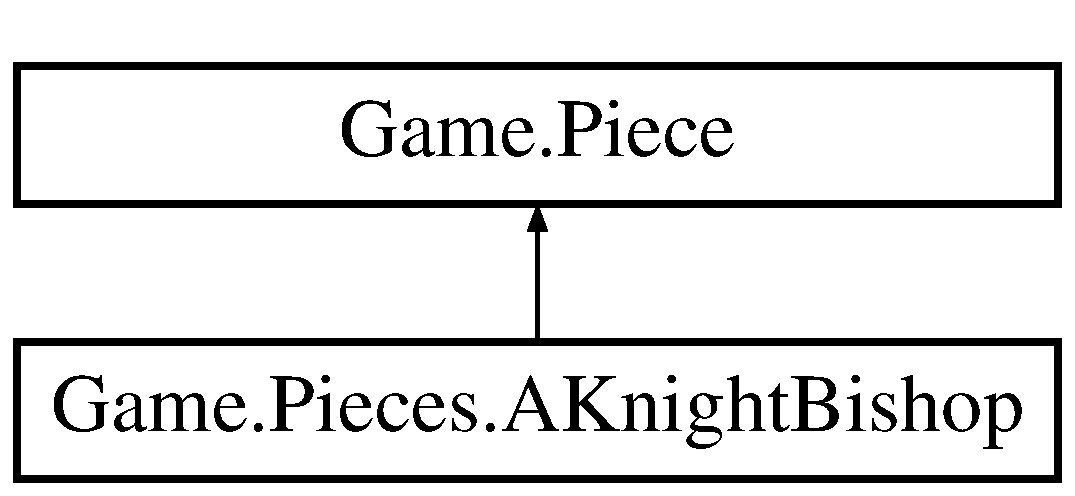
\includegraphics[height=2.000000cm]{class_game_1_1_pieces_1_1_a_knight_bishop}
\end{center}
\end{figure}
\subsection*{Public Member Functions}
\begin{DoxyCompactItemize}
\item 
\hyperlink{class_game_1_1_pieces_1_1_a_knight_bishop_a687eef276ded4074c834802d826f729c}{A\+Knight\+Bishop} (int X, int Y, int c, \hyperlink{class_game_1_1_player}{Player} owner)
\item 
Array\+List$<$ \hyperlink{class_game_1_1_location}{Location} $>$ \hyperlink{class_game_1_1_pieces_1_1_a_knight_bishop_a5f32dd9226cfeef33dabefbe0b26f415}{explore\+\_\+possible\+\_\+positions} (\hyperlink{class_game_1_1_location}{Location} location, \hyperlink{class_game_1_1_chess_board}{Chess\+Board} chess\+Board)
\end{DoxyCompactItemize}
\subsection*{Additional Inherited Members}


\subsection{Constructor \& Destructor Documentation}
\mbox{\Hypertarget{class_game_1_1_pieces_1_1_a_knight_bishop_a687eef276ded4074c834802d826f729c}\label{class_game_1_1_pieces_1_1_a_knight_bishop_a687eef276ded4074c834802d826f729c}} 
\index{Game\+::\+Pieces\+::\+A\+Knight\+Bishop@{Game\+::\+Pieces\+::\+A\+Knight\+Bishop}!A\+Knight\+Bishop@{A\+Knight\+Bishop}}
\index{A\+Knight\+Bishop@{A\+Knight\+Bishop}!Game\+::\+Pieces\+::\+A\+Knight\+Bishop@{Game\+::\+Pieces\+::\+A\+Knight\+Bishop}}
\subsubsection{\texorpdfstring{A\+Knight\+Bishop()}{AKnightBishop()}}
{\footnotesize\ttfamily Game.\+Pieces.\+A\+Knight\+Bishop.\+A\+Knight\+Bishop (\begin{DoxyParamCaption}\item[{int}]{X,  }\item[{int}]{Y,  }\item[{int}]{c,  }\item[{\hyperlink{class_game_1_1_player}{Player}}]{owner }\end{DoxyParamCaption})\hspace{0.3cm}{\ttfamily [inline]}}

Constructor.


\begin{DoxyParams}{Parameters}
{\em c} & color of piece \\
\hline
{\em X} & X coordinate \\
\hline
{\em Y} & y coordinate \\
\hline
{\em owner} & is the owner of the piece \\
\hline
\end{DoxyParams}


\subsection{Member Function Documentation}
\mbox{\Hypertarget{class_game_1_1_pieces_1_1_a_knight_bishop_a5f32dd9226cfeef33dabefbe0b26f415}\label{class_game_1_1_pieces_1_1_a_knight_bishop_a5f32dd9226cfeef33dabefbe0b26f415}} 
\index{Game\+::\+Pieces\+::\+A\+Knight\+Bishop@{Game\+::\+Pieces\+::\+A\+Knight\+Bishop}!explore\+\_\+possible\+\_\+positions@{explore\+\_\+possible\+\_\+positions}}
\index{explore\+\_\+possible\+\_\+positions@{explore\+\_\+possible\+\_\+positions}!Game\+::\+Pieces\+::\+A\+Knight\+Bishop@{Game\+::\+Pieces\+::\+A\+Knight\+Bishop}}
\subsubsection{\texorpdfstring{explore\+\_\+possible\+\_\+positions()}{explore\_possible\_positions()}}
{\footnotesize\ttfamily Array\+List$<$\hyperlink{class_game_1_1_location}{Location}$>$ Game.\+Pieces.\+A\+Knight\+Bishop.\+explore\+\_\+possible\+\_\+positions (\begin{DoxyParamCaption}\item[{\hyperlink{class_game_1_1_location}{Location}}]{location,  }\item[{\hyperlink{class_game_1_1_chess_board}{Chess\+Board}}]{chess\+Board }\end{DoxyParamCaption})\hspace{0.3cm}{\ttfamily [inline]}}

Explores all options for movement from location.


\begin{DoxyParams}{Parameters}
{\em location} & location from where we want to explore. \\
\hline
{\em chess\+Board} & is the chess board we are working on. \\
\hline
\end{DoxyParams}


The documentation for this class was generated from the following file\+:\begin{DoxyCompactItemize}
\item 
src/\+Game/\+Pieces/A\+Knight\+Bishop.\+java\end{DoxyCompactItemize}

\hypertarget{class_tests_1_1_a_knight_bishop_test}{}\section{Tests.\+A\+Knight\+Bishop\+Test Class Reference}
\label{class_tests_1_1_a_knight_bishop_test}\index{Tests.\+A\+Knight\+Bishop\+Test@{Tests.\+A\+Knight\+Bishop\+Test}}
\subsection*{Public Member Functions}
\begin{DoxyCompactItemize}
\item 
void \hyperlink{class_tests_1_1_a_knight_bishop_test_a3804ee93d28784f6c05de9de3d471f23}{can\+Move\+To\+Adjacent\+Cell\+Test} ()  throws Exception 
\item 
void \hyperlink{class_tests_1_1_a_knight_bishop_test_a9e2fdb709b6ade91bf1799f1df5ef3da}{can\+Move\+To\+Diagonal\+Cell\+Test} ()  throws Exception 
\item 
void \hyperlink{class_tests_1_1_a_knight_bishop_test_ad7f78f2a16180ec51850bb052971c903}{explore\+\_\+possible\+\_\+positions\+All\+Test} ()  throws Exception 
\item 
void \hyperlink{class_tests_1_1_a_knight_bishop_test_af78327139c271d70d6ff8f2047b24444}{explore\+\_\+possible\+\_\+positions\+Block\+Capture\+Test} ()  throws Exception 
\end{DoxyCompactItemize}


\subsection{Member Function Documentation}
\mbox{\Hypertarget{class_tests_1_1_a_knight_bishop_test_a3804ee93d28784f6c05de9de3d471f23}\label{class_tests_1_1_a_knight_bishop_test_a3804ee93d28784f6c05de9de3d471f23}} 
\index{Tests\+::\+A\+Knight\+Bishop\+Test@{Tests\+::\+A\+Knight\+Bishop\+Test}!can\+Move\+To\+Adjacent\+Cell\+Test@{can\+Move\+To\+Adjacent\+Cell\+Test}}
\index{can\+Move\+To\+Adjacent\+Cell\+Test@{can\+Move\+To\+Adjacent\+Cell\+Test}!Tests\+::\+A\+Knight\+Bishop\+Test@{Tests\+::\+A\+Knight\+Bishop\+Test}}
\subsubsection{\texorpdfstring{can\+Move\+To\+Adjacent\+Cell\+Test()}{canMoveToAdjacentCellTest()}}
{\footnotesize\ttfamily void Tests.\+A\+Knight\+Bishop\+Test.\+can\+Move\+To\+Adjacent\+Cell\+Test (\begin{DoxyParamCaption}{ }\end{DoxyParamCaption}) throws Exception\hspace{0.3cm}{\ttfamily [inline]}}

Check if Bishop can move to adjacent piece. Should return false. \mbox{\Hypertarget{class_tests_1_1_a_knight_bishop_test_a9e2fdb709b6ade91bf1799f1df5ef3da}\label{class_tests_1_1_a_knight_bishop_test_a9e2fdb709b6ade91bf1799f1df5ef3da}} 
\index{Tests\+::\+A\+Knight\+Bishop\+Test@{Tests\+::\+A\+Knight\+Bishop\+Test}!can\+Move\+To\+Diagonal\+Cell\+Test@{can\+Move\+To\+Diagonal\+Cell\+Test}}
\index{can\+Move\+To\+Diagonal\+Cell\+Test@{can\+Move\+To\+Diagonal\+Cell\+Test}!Tests\+::\+A\+Knight\+Bishop\+Test@{Tests\+::\+A\+Knight\+Bishop\+Test}}
\subsubsection{\texorpdfstring{can\+Move\+To\+Diagonal\+Cell\+Test()}{canMoveToDiagonalCellTest()}}
{\footnotesize\ttfamily void Tests.\+A\+Knight\+Bishop\+Test.\+can\+Move\+To\+Diagonal\+Cell\+Test (\begin{DoxyParamCaption}{ }\end{DoxyParamCaption}) throws Exception\hspace{0.3cm}{\ttfamily [inline]}}

Check if Bishop can move to diagonal piece. Should return true. \mbox{\Hypertarget{class_tests_1_1_a_knight_bishop_test_ad7f78f2a16180ec51850bb052971c903}\label{class_tests_1_1_a_knight_bishop_test_ad7f78f2a16180ec51850bb052971c903}} 
\index{Tests\+::\+A\+Knight\+Bishop\+Test@{Tests\+::\+A\+Knight\+Bishop\+Test}!explore\+\_\+possible\+\_\+positions\+All\+Test@{explore\+\_\+possible\+\_\+positions\+All\+Test}}
\index{explore\+\_\+possible\+\_\+positions\+All\+Test@{explore\+\_\+possible\+\_\+positions\+All\+Test}!Tests\+::\+A\+Knight\+Bishop\+Test@{Tests\+::\+A\+Knight\+Bishop\+Test}}
\subsubsection{\texorpdfstring{explore\+\_\+possible\+\_\+positions\+All\+Test()}{explore\_possible\_positionsAllTest()}}
{\footnotesize\ttfamily void Tests.\+A\+Knight\+Bishop\+Test.\+explore\+\_\+possible\+\_\+positions\+All\+Test (\begin{DoxyParamCaption}{ }\end{DoxyParamCaption}) throws Exception\hspace{0.3cm}{\ttfamily [inline]}}

Return all the places that a Bishop can go from a position with no other pieces on board. \mbox{\Hypertarget{class_tests_1_1_a_knight_bishop_test_af78327139c271d70d6ff8f2047b24444}\label{class_tests_1_1_a_knight_bishop_test_af78327139c271d70d6ff8f2047b24444}} 
\index{Tests\+::\+A\+Knight\+Bishop\+Test@{Tests\+::\+A\+Knight\+Bishop\+Test}!explore\+\_\+possible\+\_\+positions\+Block\+Capture\+Test@{explore\+\_\+possible\+\_\+positions\+Block\+Capture\+Test}}
\index{explore\+\_\+possible\+\_\+positions\+Block\+Capture\+Test@{explore\+\_\+possible\+\_\+positions\+Block\+Capture\+Test}!Tests\+::\+A\+Knight\+Bishop\+Test@{Tests\+::\+A\+Knight\+Bishop\+Test}}
\subsubsection{\texorpdfstring{explore\+\_\+possible\+\_\+positions\+Block\+Capture\+Test()}{explore\_possible\_positionsBlockCaptureTest()}}
{\footnotesize\ttfamily void Tests.\+A\+Knight\+Bishop\+Test.\+explore\+\_\+possible\+\_\+positions\+Block\+Capture\+Test (\begin{DoxyParamCaption}{ }\end{DoxyParamCaption}) throws Exception\hspace{0.3cm}{\ttfamily [inline]}}

Return all the places that a Bishop can go from a position with some pieces on board. 

The documentation for this class was generated from the following file\+:\begin{DoxyCompactItemize}
\item 
src/\+Tests/A\+Knight\+Bishop\+Test.\+java\end{DoxyCompactItemize}

\hypertarget{class_game_1_1_pieces_1_1_bishop}{}\section{Game.\+Pieces.\+Bishop Class Reference}
\label{class_game_1_1_pieces_1_1_bishop}\index{Game.\+Pieces.\+Bishop@{Game.\+Pieces.\+Bishop}}
Inheritance diagram for Game.\+Pieces.\+Bishop\+:\begin{figure}[H]
\begin{center}
\leavevmode
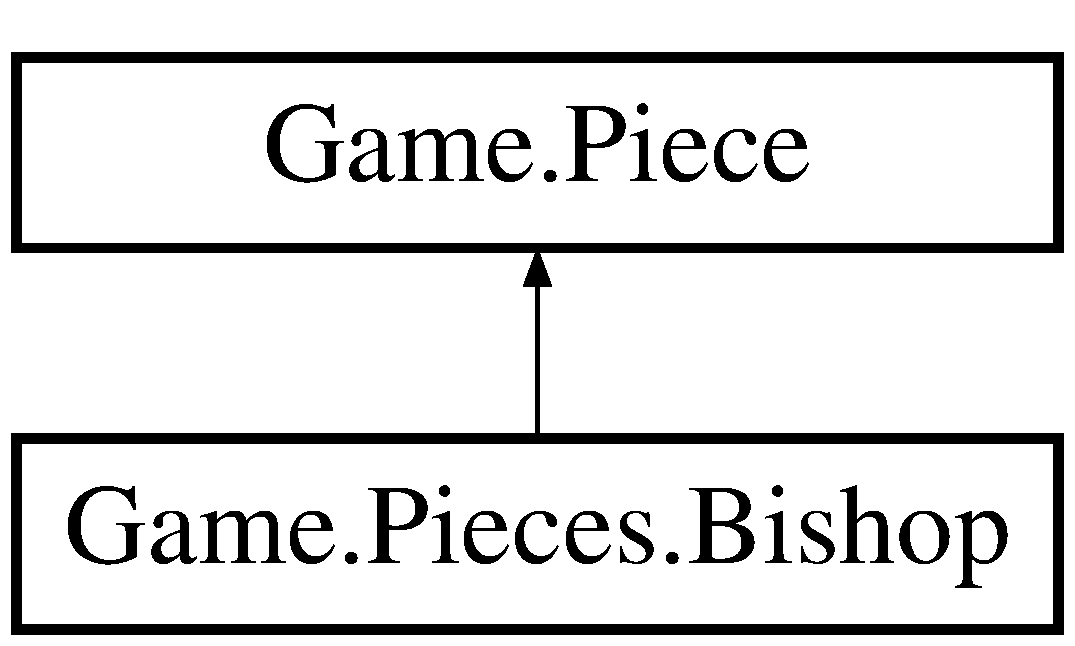
\includegraphics[height=2.000000cm]{class_game_1_1_pieces_1_1_bishop}
\end{center}
\end{figure}
\subsection*{Public Member Functions}
\begin{DoxyCompactItemize}
\item 
\hyperlink{class_game_1_1_pieces_1_1_bishop_a45e6ea33dbe889b2a5b4fb5e9f98ef2f}{Bishop} (int X, int Y, int c, \hyperlink{class_game_1_1_player}{Player} owner)
\item 
Array\+List$<$ \hyperlink{class_game_1_1_location}{Location} $>$ \hyperlink{class_game_1_1_pieces_1_1_bishop_ae20890bce6010a38c8925f02c2881c95}{explore\+\_\+possible\+\_\+positions} (\hyperlink{class_game_1_1_location}{Location} location, \hyperlink{class_game_1_1_chess_board}{Chess\+Board} chess\+Board)
\end{DoxyCompactItemize}
\subsection*{Additional Inherited Members}


\subsection{Constructor \& Destructor Documentation}
\mbox{\Hypertarget{class_game_1_1_pieces_1_1_bishop_a45e6ea33dbe889b2a5b4fb5e9f98ef2f}\label{class_game_1_1_pieces_1_1_bishop_a45e6ea33dbe889b2a5b4fb5e9f98ef2f}} 
\index{Game\+::\+Pieces\+::\+Bishop@{Game\+::\+Pieces\+::\+Bishop}!Bishop@{Bishop}}
\index{Bishop@{Bishop}!Game\+::\+Pieces\+::\+Bishop@{Game\+::\+Pieces\+::\+Bishop}}
\subsubsection{\texorpdfstring{Bishop()}{Bishop()}}
{\footnotesize\ttfamily Game.\+Pieces.\+Bishop.\+Bishop (\begin{DoxyParamCaption}\item[{int}]{X,  }\item[{int}]{Y,  }\item[{int}]{c,  }\item[{\hyperlink{class_game_1_1_player}{Player}}]{owner }\end{DoxyParamCaption})\hspace{0.3cm}{\ttfamily [inline]}}

Constructor. 
\begin{DoxyParams}{Parameters}
{\em c} & color of piece \\
\hline
{\em X} & X coordinate \\
\hline
{\em Y} & y coordinate \\
\hline
{\em owner} & is the owner of the piece \\
\hline
\end{DoxyParams}


\subsection{Member Function Documentation}
\mbox{\Hypertarget{class_game_1_1_pieces_1_1_bishop_ae20890bce6010a38c8925f02c2881c95}\label{class_game_1_1_pieces_1_1_bishop_ae20890bce6010a38c8925f02c2881c95}} 
\index{Game\+::\+Pieces\+::\+Bishop@{Game\+::\+Pieces\+::\+Bishop}!explore\+\_\+possible\+\_\+positions@{explore\+\_\+possible\+\_\+positions}}
\index{explore\+\_\+possible\+\_\+positions@{explore\+\_\+possible\+\_\+positions}!Game\+::\+Pieces\+::\+Bishop@{Game\+::\+Pieces\+::\+Bishop}}
\subsubsection{\texorpdfstring{explore\+\_\+possible\+\_\+positions()}{explore\_possible\_positions()}}
{\footnotesize\ttfamily Array\+List$<$\hyperlink{class_game_1_1_location}{Location}$>$ Game.\+Pieces.\+Bishop.\+explore\+\_\+possible\+\_\+positions (\begin{DoxyParamCaption}\item[{\hyperlink{class_game_1_1_location}{Location}}]{location,  }\item[{\hyperlink{class_game_1_1_chess_board}{Chess\+Board}}]{chess\+Board }\end{DoxyParamCaption})\hspace{0.3cm}{\ttfamily [inline]}}

Explores all options for movement from location. 
\begin{DoxyParams}{Parameters}
{\em location} & location from where we want to explore. \\
\hline
{\em chess\+Board} & is the chess board we are working on. \\
\hline
\end{DoxyParams}


The documentation for this class was generated from the following file\+:\begin{DoxyCompactItemize}
\item 
src/\+Game/\+Pieces/Bishop.\+java\end{DoxyCompactItemize}

\hypertarget{class_tests_1_1_bishop_test}{}\section{Tests.\+Bishop\+Test Class Reference}
\label{class_tests_1_1_bishop_test}\index{Tests.\+Bishop\+Test@{Tests.\+Bishop\+Test}}
\subsection*{Public Member Functions}
\begin{DoxyCompactItemize}
\item 
void \hyperlink{class_tests_1_1_bishop_test_af8320bc069c8e9f0d2463a046161a174}{can\+Move\+To\+Adjacent\+Cell\+Test} ()  throws Exception 
\item 
void \hyperlink{class_tests_1_1_bishop_test_ad994f25fbfd9195cfb06b0dfac9c4958}{can\+Move\+To\+Diagonal\+Cell\+Test} ()  throws Exception 
\item 
void \hyperlink{class_tests_1_1_bishop_test_a39c7fec14bfa1fe60b4a669d3f52d6b3}{explore\+\_\+possible\+\_\+positions\+All\+Test} ()  throws Exception 
\item 
void \hyperlink{class_tests_1_1_bishop_test_a3da32d2c9bd46cef51386f999bb02e64}{explore\+\_\+possible\+\_\+positions\+Block\+Capture\+Test} ()  throws Exception 
\end{DoxyCompactItemize}


\subsection{Member Function Documentation}
\mbox{\Hypertarget{class_tests_1_1_bishop_test_af8320bc069c8e9f0d2463a046161a174}\label{class_tests_1_1_bishop_test_af8320bc069c8e9f0d2463a046161a174}} 
\index{Tests\+::\+Bishop\+Test@{Tests\+::\+Bishop\+Test}!can\+Move\+To\+Adjacent\+Cell\+Test@{can\+Move\+To\+Adjacent\+Cell\+Test}}
\index{can\+Move\+To\+Adjacent\+Cell\+Test@{can\+Move\+To\+Adjacent\+Cell\+Test}!Tests\+::\+Bishop\+Test@{Tests\+::\+Bishop\+Test}}
\subsubsection{\texorpdfstring{can\+Move\+To\+Adjacent\+Cell\+Test()}{canMoveToAdjacentCellTest()}}
{\footnotesize\ttfamily void Tests.\+Bishop\+Test.\+can\+Move\+To\+Adjacent\+Cell\+Test (\begin{DoxyParamCaption}{ }\end{DoxyParamCaption}) throws Exception\hspace{0.3cm}{\ttfamily [inline]}}

Check if Bishop can move to adjacent piece. Should return false. \mbox{\Hypertarget{class_tests_1_1_bishop_test_ad994f25fbfd9195cfb06b0dfac9c4958}\label{class_tests_1_1_bishop_test_ad994f25fbfd9195cfb06b0dfac9c4958}} 
\index{Tests\+::\+Bishop\+Test@{Tests\+::\+Bishop\+Test}!can\+Move\+To\+Diagonal\+Cell\+Test@{can\+Move\+To\+Diagonal\+Cell\+Test}}
\index{can\+Move\+To\+Diagonal\+Cell\+Test@{can\+Move\+To\+Diagonal\+Cell\+Test}!Tests\+::\+Bishop\+Test@{Tests\+::\+Bishop\+Test}}
\subsubsection{\texorpdfstring{can\+Move\+To\+Diagonal\+Cell\+Test()}{canMoveToDiagonalCellTest()}}
{\footnotesize\ttfamily void Tests.\+Bishop\+Test.\+can\+Move\+To\+Diagonal\+Cell\+Test (\begin{DoxyParamCaption}{ }\end{DoxyParamCaption}) throws Exception\hspace{0.3cm}{\ttfamily [inline]}}

Check if Bishop can move to diagonal piece. Should return true. \mbox{\Hypertarget{class_tests_1_1_bishop_test_a39c7fec14bfa1fe60b4a669d3f52d6b3}\label{class_tests_1_1_bishop_test_a39c7fec14bfa1fe60b4a669d3f52d6b3}} 
\index{Tests\+::\+Bishop\+Test@{Tests\+::\+Bishop\+Test}!explore\+\_\+possible\+\_\+positions\+All\+Test@{explore\+\_\+possible\+\_\+positions\+All\+Test}}
\index{explore\+\_\+possible\+\_\+positions\+All\+Test@{explore\+\_\+possible\+\_\+positions\+All\+Test}!Tests\+::\+Bishop\+Test@{Tests\+::\+Bishop\+Test}}
\subsubsection{\texorpdfstring{explore\+\_\+possible\+\_\+positions\+All\+Test()}{explore\_possible\_positionsAllTest()}}
{\footnotesize\ttfamily void Tests.\+Bishop\+Test.\+explore\+\_\+possible\+\_\+positions\+All\+Test (\begin{DoxyParamCaption}{ }\end{DoxyParamCaption}) throws Exception\hspace{0.3cm}{\ttfamily [inline]}}

Return all the places that a Bishop can go from a position with no other pieces on board. \mbox{\Hypertarget{class_tests_1_1_bishop_test_a3da32d2c9bd46cef51386f999bb02e64}\label{class_tests_1_1_bishop_test_a3da32d2c9bd46cef51386f999bb02e64}} 
\index{Tests\+::\+Bishop\+Test@{Tests\+::\+Bishop\+Test}!explore\+\_\+possible\+\_\+positions\+Block\+Capture\+Test@{explore\+\_\+possible\+\_\+positions\+Block\+Capture\+Test}}
\index{explore\+\_\+possible\+\_\+positions\+Block\+Capture\+Test@{explore\+\_\+possible\+\_\+positions\+Block\+Capture\+Test}!Tests\+::\+Bishop\+Test@{Tests\+::\+Bishop\+Test}}
\subsubsection{\texorpdfstring{explore\+\_\+possible\+\_\+positions\+Block\+Capture\+Test()}{explore\_possible\_positionsBlockCaptureTest()}}
{\footnotesize\ttfamily void Tests.\+Bishop\+Test.\+explore\+\_\+possible\+\_\+positions\+Block\+Capture\+Test (\begin{DoxyParamCaption}{ }\end{DoxyParamCaption}) throws Exception\hspace{0.3cm}{\ttfamily [inline]}}

Return all the places that a Bishop can go from a position with some pieces on board. 

The documentation for this class was generated from the following file\+:\begin{DoxyCompactItemize}
\item 
src/\+Tests/Bishop\+Test.\+java\end{DoxyCompactItemize}

\hypertarget{class_game_1_1_chess_board}{}\section{Game.\+Chess\+Board Class Reference}
\label{class_game_1_1_chess_board}\index{Game.\+Chess\+Board@{Game.\+Chess\+Board}}
\subsection*{Public Member Functions}
\begin{DoxyCompactItemize}
\item 
\hyperlink{class_game_1_1_chess_board_af03bbcf15fe65eb707758928b92556d7}{Chess\+Board} ()
\item 
\mbox{\Hypertarget{class_game_1_1_chess_board_a6cd8d8698cb3613f1ea0c6ff12ff2bad}\label{class_game_1_1_chess_board_a6cd8d8698cb3613f1ea0c6ff12ff2bad}} 
\hyperlink{class_game_1_1_player}{Player} {\bfseries get\+Player\+White} ()
\item 
\mbox{\Hypertarget{class_game_1_1_chess_board_a7e03a5285b591f072128fe7fc1afcfa0}\label{class_game_1_1_chess_board_a7e03a5285b591f072128fe7fc1afcfa0}} 
\hyperlink{class_game_1_1_player}{Player} {\bfseries get\+Player\+Black} ()
\item 
void \hyperlink{class_game_1_1_chess_board_a56eeb955a8ced4615f314e96e1d0fb0d}{set\+Board\+Afresh} ()
\item 
void \hyperlink{class_game_1_1_chess_board_ac47067200b06bc4d11ca660c7a409956}{print\+Board} (Hash\+Map$<$ \hyperlink{class_game_1_1_location}{Location}, \hyperlink{class_game_1_1_piece}{Piece} $>$ board)
\item 
void \hyperlink{class_game_1_1_chess_board_abe952ff3498a25cf31170ff416ca6954}{print\+Board\+Print} ()
\item 
\hyperlink{class_game_1_1_location}{Location} \hyperlink{class_game_1_1_chess_board_a021ffe2d9253de4c5a59e58c6dd52730}{find\+\_\+location} (int x, int y)
\item 
void \hyperlink{class_game_1_1_chess_board_a9ec942366d90c6dca4c1da936e040474}{set\+Up\+Start\+Board} (\hyperlink{class_game_1_1_chess_board}{Chess\+Board} chess\+Board)
\item 
\mbox{\Hypertarget{class_game_1_1_chess_board_a3292913ce4081ea271aba5295cafaf41}\label{class_game_1_1_chess_board_a3292913ce4081ea271aba5295cafaf41}} 
int \mbox{[}$\,$\mbox{]}\mbox{[}$\,$\mbox{]} {\bfseries get\+Board\+Print} ()
\item 
\mbox{\Hypertarget{class_game_1_1_chess_board_ac66d60d971579df2d51acfb2796f6bda}\label{class_game_1_1_chess_board_ac66d60d971579df2d51acfb2796f6bda}} 
Hash\+Map$<$ \hyperlink{class_game_1_1_location}{Location}, \hyperlink{class_game_1_1_piece}{Piece} $>$ {\bfseries get\+Board} ()
\item 
boolean \hyperlink{class_game_1_1_chess_board_a79832c1dee410398129a1d2365819836}{checkmated} (\hyperlink{class_game_1_1_player}{Player} player, \hyperlink{class_game_1_1_chess_board}{Chess\+Board} chess\+Board)
\item 
boolean \hyperlink{class_game_1_1_chess_board_a7a2ec0cc1f431ee502561c18a53a80cf}{in\+Stalemate} (\hyperlink{class_game_1_1_chess_board}{Chess\+Board} chess\+Board)
\item 
boolean \hyperlink{class_game_1_1_chess_board_a7176cdb726816d1a5ce1aabd01c7f706}{in\+Check} (\hyperlink{class_game_1_1_player}{Player} player, \hyperlink{class_game_1_1_chess_board}{Chess\+Board} chess\+Board)
\item 
\hyperlink{class_game_1_1_piece}{Piece} \hyperlink{class_game_1_1_chess_board_af7f79327e5c2e5ed8f60715736e684d2}{get\+King} (\hyperlink{class_game_1_1_player}{Player} player)
\item 
\hyperlink{class_game_1_1_player}{Player} \hyperlink{class_game_1_1_chess_board_af26bbaf05bffe9f911e10ad3e2843c6a}{get\+Current\+Player} ()
\item 
\hyperlink{class_game_1_1_player}{Player} \hyperlink{class_game_1_1_chess_board_a3d8adea17ddbb65aa9e527e711f80c51}{get\+Other\+Player} (\hyperlink{class_game_1_1_player}{Player} player)
\item 
\mbox{\Hypertarget{class_game_1_1_chess_board_a379b1fc092ee1ff5a14fac5461ae0112}\label{class_game_1_1_chess_board_a379b1fc092ee1ff5a14fac5461ae0112}} 
void {\bfseries place\+Piece} (\hyperlink{class_game_1_1_piece}{Piece} piece)
\item 
\mbox{\Hypertarget{class_game_1_1_chess_board_a61728334465aa8a90a32fe141d67b99d}\label{class_game_1_1_chess_board_a61728334465aa8a90a32fe141d67b99d}} 
boolean {\bfseries is\+On\+Board} (int x, int y)
\item 
\mbox{\Hypertarget{class_game_1_1_chess_board_a14bb6eb4e1b62827762a9089bba60621}\label{class_game_1_1_chess_board_a14bb6eb4e1b62827762a9089bba60621}} 
int {\bfseries get\+Ranks} ()
\item 
\mbox{\Hypertarget{class_game_1_1_chess_board_a32690c9ed46310a3b1cb9321e7e4680b}\label{class_game_1_1_chess_board_a32690c9ed46310a3b1cb9321e7e4680b}} 
int {\bfseries get\+Files} ()
\end{DoxyCompactItemize}


\subsection{Constructor \& Destructor Documentation}
\mbox{\Hypertarget{class_game_1_1_chess_board_af03bbcf15fe65eb707758928b92556d7}\label{class_game_1_1_chess_board_af03bbcf15fe65eb707758928b92556d7}} 
\index{Game\+::\+Chess\+Board@{Game\+::\+Chess\+Board}!Chess\+Board@{Chess\+Board}}
\index{Chess\+Board@{Chess\+Board}!Game\+::\+Chess\+Board@{Game\+::\+Chess\+Board}}
\subsubsection{\texorpdfstring{Chess\+Board()}{ChessBoard()}}
{\footnotesize\ttfamily Game.\+Chess\+Board.\+Chess\+Board (\begin{DoxyParamCaption}{ }\end{DoxyParamCaption})\hspace{0.3cm}{\ttfamily [inline]}}

Constructor for \hyperlink{class_game_1_1_chess_board}{Chess\+Board}. Intended for the board data structures and checking if won or not. 

\subsection{Member Function Documentation}
\mbox{\Hypertarget{class_game_1_1_chess_board_a79832c1dee410398129a1d2365819836}\label{class_game_1_1_chess_board_a79832c1dee410398129a1d2365819836}} 
\index{Game\+::\+Chess\+Board@{Game\+::\+Chess\+Board}!checkmated@{checkmated}}
\index{checkmated@{checkmated}!Game\+::\+Chess\+Board@{Game\+::\+Chess\+Board}}
\subsubsection{\texorpdfstring{checkmated()}{checkmated()}}
{\footnotesize\ttfamily boolean Game.\+Chess\+Board.\+checkmated (\begin{DoxyParamCaption}\item[{\hyperlink{class_game_1_1_player}{Player}}]{player,  }\item[{\hyperlink{class_game_1_1_chess_board}{Chess\+Board}}]{chess\+Board }\end{DoxyParamCaption})\hspace{0.3cm}{\ttfamily [inline]}}

Checks whether player is check mated. 
\begin{DoxyParams}{Parameters}
{\em chess\+Board} & board to check players status on \\
\hline
{\em player} & player to check the status of \\
\hline
\end{DoxyParams}
\begin{DoxyReturn}{Returns}
Whether the player has been checkmated. 
\end{DoxyReturn}
\mbox{\Hypertarget{class_game_1_1_chess_board_a021ffe2d9253de4c5a59e58c6dd52730}\label{class_game_1_1_chess_board_a021ffe2d9253de4c5a59e58c6dd52730}} 
\index{Game\+::\+Chess\+Board@{Game\+::\+Chess\+Board}!find\+\_\+location@{find\+\_\+location}}
\index{find\+\_\+location@{find\+\_\+location}!Game\+::\+Chess\+Board@{Game\+::\+Chess\+Board}}
\subsubsection{\texorpdfstring{find\+\_\+location()}{find\_location()}}
{\footnotesize\ttfamily \hyperlink{class_game_1_1_location}{Location} Game.\+Chess\+Board.\+find\+\_\+location (\begin{DoxyParamCaption}\item[{int}]{x,  }\item[{int}]{y }\end{DoxyParamCaption})\hspace{0.3cm}{\ttfamily [inline]}}

Finds the location given x and y coordinates. 
\begin{DoxyParams}{Parameters}
{\em x} & is the x coordinate \\
\hline
{\em x} & is the x coordinate \\
\hline
\end{DoxyParams}
\mbox{\Hypertarget{class_game_1_1_chess_board_af26bbaf05bffe9f911e10ad3e2843c6a}\label{class_game_1_1_chess_board_af26bbaf05bffe9f911e10ad3e2843c6a}} 
\index{Game\+::\+Chess\+Board@{Game\+::\+Chess\+Board}!get\+Current\+Player@{get\+Current\+Player}}
\index{get\+Current\+Player@{get\+Current\+Player}!Game\+::\+Chess\+Board@{Game\+::\+Chess\+Board}}
\subsubsection{\texorpdfstring{get\+Current\+Player()}{getCurrentPlayer()}}
{\footnotesize\ttfamily \hyperlink{class_game_1_1_player}{Player} Game.\+Chess\+Board.\+get\+Current\+Player (\begin{DoxyParamCaption}{ }\end{DoxyParamCaption})\hspace{0.3cm}{\ttfamily [inline]}}

Returns current player \mbox{\Hypertarget{class_game_1_1_chess_board_af7f79327e5c2e5ed8f60715736e684d2}\label{class_game_1_1_chess_board_af7f79327e5c2e5ed8f60715736e684d2}} 
\index{Game\+::\+Chess\+Board@{Game\+::\+Chess\+Board}!get\+King@{get\+King}}
\index{get\+King@{get\+King}!Game\+::\+Chess\+Board@{Game\+::\+Chess\+Board}}
\subsubsection{\texorpdfstring{get\+King()}{getKing()}}
{\footnotesize\ttfamily \hyperlink{class_game_1_1_piece}{Piece} Game.\+Chess\+Board.\+get\+King (\begin{DoxyParamCaption}\item[{\hyperlink{class_game_1_1_player}{Player}}]{player }\end{DoxyParamCaption})\hspace{0.3cm}{\ttfamily [inline]}}

Gets king piece 
\begin{DoxyParams}{Parameters}
{\em player} & player to check the status of \\
\hline
\end{DoxyParams}
\begin{DoxyReturn}{Returns}
King piece of player 
\end{DoxyReturn}
\mbox{\Hypertarget{class_game_1_1_chess_board_a3d8adea17ddbb65aa9e527e711f80c51}\label{class_game_1_1_chess_board_a3d8adea17ddbb65aa9e527e711f80c51}} 
\index{Game\+::\+Chess\+Board@{Game\+::\+Chess\+Board}!get\+Other\+Player@{get\+Other\+Player}}
\index{get\+Other\+Player@{get\+Other\+Player}!Game\+::\+Chess\+Board@{Game\+::\+Chess\+Board}}
\subsubsection{\texorpdfstring{get\+Other\+Player()}{getOtherPlayer()}}
{\footnotesize\ttfamily \hyperlink{class_game_1_1_player}{Player} Game.\+Chess\+Board.\+get\+Other\+Player (\begin{DoxyParamCaption}\item[{\hyperlink{class_game_1_1_player}{Player}}]{player }\end{DoxyParamCaption})\hspace{0.3cm}{\ttfamily [inline]}}

Returns the other player \mbox{\Hypertarget{class_game_1_1_chess_board_a7176cdb726816d1a5ce1aabd01c7f706}\label{class_game_1_1_chess_board_a7176cdb726816d1a5ce1aabd01c7f706}} 
\index{Game\+::\+Chess\+Board@{Game\+::\+Chess\+Board}!in\+Check@{in\+Check}}
\index{in\+Check@{in\+Check}!Game\+::\+Chess\+Board@{Game\+::\+Chess\+Board}}
\subsubsection{\texorpdfstring{in\+Check()}{inCheck()}}
{\footnotesize\ttfamily boolean Game.\+Chess\+Board.\+in\+Check (\begin{DoxyParamCaption}\item[{\hyperlink{class_game_1_1_player}{Player}}]{player,  }\item[{\hyperlink{class_game_1_1_chess_board}{Chess\+Board}}]{chess\+Board }\end{DoxyParamCaption})\hspace{0.3cm}{\ttfamily [inline]}}

Checks whether player is in check. 
\begin{DoxyParams}{Parameters}
{\em chess\+Board} & board to check players status on \\
\hline
{\em player} & player to check the status of \\
\hline
\end{DoxyParams}
\begin{DoxyReturn}{Returns}
Whether the player is in check. 
\end{DoxyReturn}
\mbox{\Hypertarget{class_game_1_1_chess_board_a7a2ec0cc1f431ee502561c18a53a80cf}\label{class_game_1_1_chess_board_a7a2ec0cc1f431ee502561c18a53a80cf}} 
\index{Game\+::\+Chess\+Board@{Game\+::\+Chess\+Board}!in\+Stalemate@{in\+Stalemate}}
\index{in\+Stalemate@{in\+Stalemate}!Game\+::\+Chess\+Board@{Game\+::\+Chess\+Board}}
\subsubsection{\texorpdfstring{in\+Stalemate()}{inStalemate()}}
{\footnotesize\ttfamily boolean Game.\+Chess\+Board.\+in\+Stalemate (\begin{DoxyParamCaption}\item[{\hyperlink{class_game_1_1_chess_board}{Chess\+Board}}]{chess\+Board }\end{DoxyParamCaption})\hspace{0.3cm}{\ttfamily [inline]}}

If the player who\textquotesingle{}s turn it currently is is not in check and cannot move, return true 
\begin{DoxyParams}{Parameters}
{\em chess\+Board} & board to check players status on \\
\hline
\end{DoxyParams}
\begin{DoxyReturn}{Returns}
is the game in stalemate 
\end{DoxyReturn}
\mbox{\Hypertarget{class_game_1_1_chess_board_ac47067200b06bc4d11ca660c7a409956}\label{class_game_1_1_chess_board_ac47067200b06bc4d11ca660c7a409956}} 
\index{Game\+::\+Chess\+Board@{Game\+::\+Chess\+Board}!print\+Board@{print\+Board}}
\index{print\+Board@{print\+Board}!Game\+::\+Chess\+Board@{Game\+::\+Chess\+Board}}
\subsubsection{\texorpdfstring{print\+Board()}{printBoard()}}
{\footnotesize\ttfamily void Game.\+Chess\+Board.\+print\+Board (\begin{DoxyParamCaption}\item[{Hash\+Map$<$ \hyperlink{class_game_1_1_location}{Location}, \hyperlink{class_game_1_1_piece}{Piece} $>$}]{board }\end{DoxyParamCaption})\hspace{0.3cm}{\ttfamily [inline]}}

Prints the board with data structure Hash\+Map$<$\+Location, Piece$>$ board. 
\begin{DoxyParams}{Parameters}
{\em board} & the data structure which contains pieces at certain locations. \\
\hline
\end{DoxyParams}
\mbox{\Hypertarget{class_game_1_1_chess_board_abe952ff3498a25cf31170ff416ca6954}\label{class_game_1_1_chess_board_abe952ff3498a25cf31170ff416ca6954}} 
\index{Game\+::\+Chess\+Board@{Game\+::\+Chess\+Board}!print\+Board\+Print@{print\+Board\+Print}}
\index{print\+Board\+Print@{print\+Board\+Print}!Game\+::\+Chess\+Board@{Game\+::\+Chess\+Board}}
\subsubsection{\texorpdfstring{print\+Board\+Print()}{printBoardPrint()}}
{\footnotesize\ttfamily void Game.\+Chess\+Board.\+print\+Board\+Print (\begin{DoxyParamCaption}{ }\end{DoxyParamCaption})\hspace{0.3cm}{\ttfamily [inline]}}

Prints the board with data structure int\mbox{[}\mbox{]}\mbox{[}\mbox{]} board. \mbox{\Hypertarget{class_game_1_1_chess_board_a56eeb955a8ced4615f314e96e1d0fb0d}\label{class_game_1_1_chess_board_a56eeb955a8ced4615f314e96e1d0fb0d}} 
\index{Game\+::\+Chess\+Board@{Game\+::\+Chess\+Board}!set\+Board\+Afresh@{set\+Board\+Afresh}}
\index{set\+Board\+Afresh@{set\+Board\+Afresh}!Game\+::\+Chess\+Board@{Game\+::\+Chess\+Board}}
\subsubsection{\texorpdfstring{set\+Board\+Afresh()}{setBoardAfresh()}}
{\footnotesize\ttfamily void Game.\+Chess\+Board.\+set\+Board\+Afresh (\begin{DoxyParamCaption}{ }\end{DoxyParamCaption})\hspace{0.3cm}{\ttfamily [inline]}}

Set the board up, Empty. \mbox{\Hypertarget{class_game_1_1_chess_board_a9ec942366d90c6dca4c1da936e040474}\label{class_game_1_1_chess_board_a9ec942366d90c6dca4c1da936e040474}} 
\index{Game\+::\+Chess\+Board@{Game\+::\+Chess\+Board}!set\+Up\+Start\+Board@{set\+Up\+Start\+Board}}
\index{set\+Up\+Start\+Board@{set\+Up\+Start\+Board}!Game\+::\+Chess\+Board@{Game\+::\+Chess\+Board}}
\subsubsection{\texorpdfstring{set\+Up\+Start\+Board()}{setUpStartBoard()}}
{\footnotesize\ttfamily void Game.\+Chess\+Board.\+set\+Up\+Start\+Board (\begin{DoxyParamCaption}\item[{\hyperlink{class_game_1_1_chess_board}{Chess\+Board}}]{chess\+Board }\end{DoxyParamCaption})\hspace{0.3cm}{\ttfamily [inline]}}

Set the board up to the initial board set up, with all data structures full of . 

The documentation for this class was generated from the following file\+:\begin{DoxyCompactItemize}
\item 
src/\+Game/Chess\+Board.\+java\end{DoxyCompactItemize}

\hypertarget{class_g_u_i_1_1_chessboard_g_u_i}{}\section{G\+U\+I.\+Chessboard\+G\+UI Class Reference}
\label{class_g_u_i_1_1_chessboard_g_u_i}\index{G\+U\+I.\+Chessboard\+G\+UI@{G\+U\+I.\+Chessboard\+G\+UI}}
Inheritance diagram for G\+U\+I.\+Chessboard\+G\+UI\+:\begin{figure}[H]
\begin{center}
\leavevmode
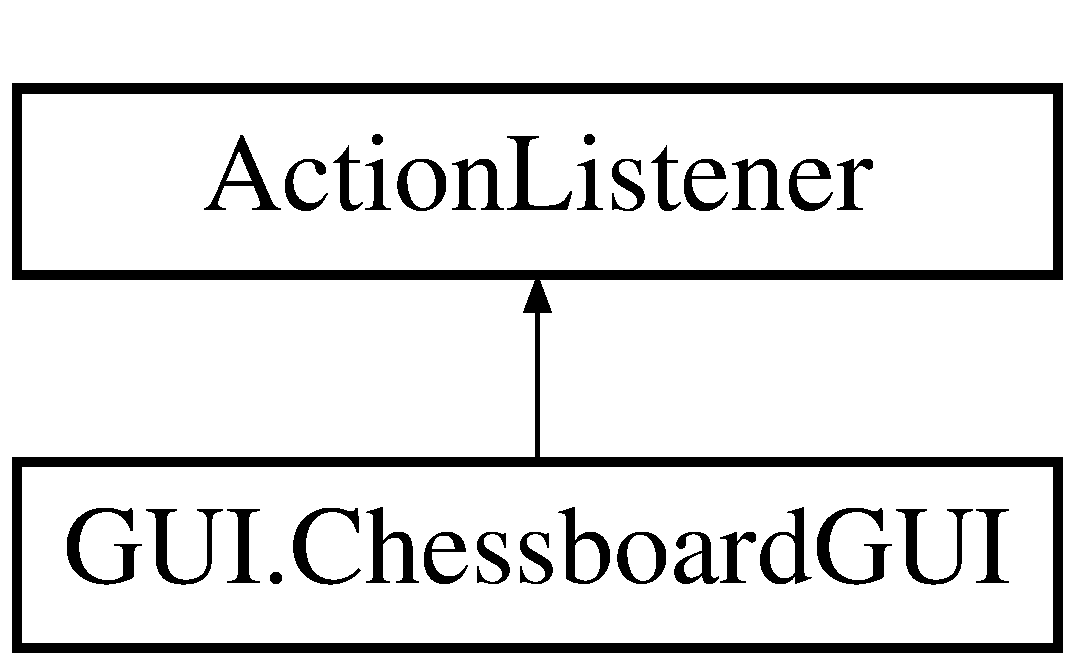
\includegraphics[height=2.000000cm]{class_g_u_i_1_1_chessboard_g_u_i}
\end{center}
\end{figure}
\subsection*{Public Member Functions}
\begin{DoxyCompactItemize}
\item 
\hyperlink{class_g_u_i_1_1_chessboard_g_u_i_a54614b37f2b48869a626ed8358719682}{Chessboard\+G\+UI} (\hyperlink{class_game_1_1_chess_board}{Chess\+Board} chess\+Data)
\item 
\mbox{\Hypertarget{class_g_u_i_1_1_chessboard_g_u_i_a83d5802a263c7a8a4a58825f1f60824f}\label{class_g_u_i_1_1_chessboard_g_u_i_a83d5802a263c7a8a4a58825f1f60824f}} 
void {\bfseries action\+Performed} (Action\+Event e)
\end{DoxyCompactItemize}
\subsection*{Static Public Member Functions}
\begin{DoxyCompactItemize}
\item 
static void \hyperlink{class_g_u_i_1_1_chessboard_g_u_i_a2ed2bd7b9e65ae8a4e92c27e76b0c14f}{main} (String args\mbox{[}$\,$\mbox{]})
\end{DoxyCompactItemize}


\subsection{Detailed Description}
This class is used to generate the G\+UI for a chess game. Currently, it is a Static G\+UI. NO moves have been implemented. 

\subsection{Constructor \& Destructor Documentation}
\mbox{\Hypertarget{class_g_u_i_1_1_chessboard_g_u_i_a54614b37f2b48869a626ed8358719682}\label{class_g_u_i_1_1_chessboard_g_u_i_a54614b37f2b48869a626ed8358719682}} 
\index{G\+U\+I\+::\+Chessboard\+G\+UI@{G\+U\+I\+::\+Chessboard\+G\+UI}!Chessboard\+G\+UI@{Chessboard\+G\+UI}}
\index{Chessboard\+G\+UI@{Chessboard\+G\+UI}!G\+U\+I\+::\+Chessboard\+G\+UI@{G\+U\+I\+::\+Chessboard\+G\+UI}}
\subsubsection{\texorpdfstring{Chessboard\+G\+U\+I()}{ChessboardGUI()}}
{\footnotesize\ttfamily G\+U\+I.\+Chessboard\+G\+U\+I.\+Chessboard\+G\+UI (\begin{DoxyParamCaption}\item[{\hyperlink{class_game_1_1_chess_board}{Chess\+Board}}]{chess\+Data }\end{DoxyParamCaption})\hspace{0.3cm}{\ttfamily [inline]}}

This is the constructor for the G\+UI for the chessboard. 
\begin{DoxyParams}{Parameters}
{\em chess\+Data} & \\
\hline
\end{DoxyParams}


\subsection{Member Function Documentation}
\mbox{\Hypertarget{class_g_u_i_1_1_chessboard_g_u_i_a2ed2bd7b9e65ae8a4e92c27e76b0c14f}\label{class_g_u_i_1_1_chessboard_g_u_i_a2ed2bd7b9e65ae8a4e92c27e76b0c14f}} 
\index{G\+U\+I\+::\+Chessboard\+G\+UI@{G\+U\+I\+::\+Chessboard\+G\+UI}!main@{main}}
\index{main@{main}!G\+U\+I\+::\+Chessboard\+G\+UI@{G\+U\+I\+::\+Chessboard\+G\+UI}}
\subsubsection{\texorpdfstring{main()}{main()}}
{\footnotesize\ttfamily static void G\+U\+I.\+Chessboard\+G\+U\+I.\+main (\begin{DoxyParamCaption}\item[{String}]{args\mbox{[}$\,$\mbox{]} }\end{DoxyParamCaption})\hspace{0.3cm}{\ttfamily [inline]}, {\ttfamily [static]}}

This is the main function where G\+UI is tested. For each test case, refer to \hyperlink{class_g_u_i_1_1_chessboard_g_u_i}{Chessboard\+G\+UI} test. Copy the function contents and run. 
\begin{DoxyParams}{Parameters}
{\em args} & \\
\hline
\end{DoxyParams}


The documentation for this class was generated from the following file\+:\begin{DoxyCompactItemize}
\item 
src/\+G\+U\+I/Chessboard\+G\+U\+I.\+java\end{DoxyCompactItemize}

\hypertarget{class_tests_1_1_chessboard_g_u_i_test}{}\section{Tests.\+Chessboard\+G\+U\+I\+Test Class Reference}
\label{class_tests_1_1_chessboard_g_u_i_test}\index{Tests.\+Chessboard\+G\+U\+I\+Test@{Tests.\+Chessboard\+G\+U\+I\+Test}}
\subsection*{Public Member Functions}
\begin{DoxyCompactItemize}
\item 
\mbox{\Hypertarget{class_tests_1_1_chessboard_g_u_i_test_a5a9da2f8c2f014f31aa34d4bb781b4ae}\label{class_tests_1_1_chessboard_g_u_i_test_a5a9da2f8c2f014f31aa34d4bb781b4ae}} 
void {\bfseries Full\+Chessboard\+G\+U\+I\+Test} ()  throws Exception 
\item 
\mbox{\Hypertarget{class_tests_1_1_chessboard_g_u_i_test_a84f66182a48f7474ef33eacaf165567d}\label{class_tests_1_1_chessboard_g_u_i_test_a84f66182a48f7474ef33eacaf165567d}} 
void {\bfseries Custom\+Piece\+Chessboard\+G\+U\+I\+Test} ()  throws Exception 
\item 
\mbox{\Hypertarget{class_tests_1_1_chessboard_g_u_i_test_ad1c574e527444b3299e7b3f3323024fe}\label{class_tests_1_1_chessboard_g_u_i_test_ad1c574e527444b3299e7b3f3323024fe}} 
void {\bfseries Checkmate\+Situation\+Chessboard\+G\+U\+I\+Test} ()  throws Exception 
\item 
\mbox{\Hypertarget{class_tests_1_1_chessboard_g_u_i_test_ab139828ce3540931f2cd2bec144df59a}\label{class_tests_1_1_chessboard_g_u_i_test_ab139828ce3540931f2cd2bec144df59a}} 
void {\bfseries Piece\+Outside\+Chessboard\+G\+U\+I\+Test} ()  throws Exception 
\item 
\mbox{\Hypertarget{class_tests_1_1_chessboard_g_u_i_test_a432558b43ad2d177d971f1da866f4462}\label{class_tests_1_1_chessboard_g_u_i_test_a432558b43ad2d177d971f1da866f4462}} 
void {\bfseries tear\+Down} ()  throws Exception 
\end{DoxyCompactItemize}


The documentation for this class was generated from the following file\+:\begin{DoxyCompactItemize}
\item 
src/\+Tests/Chessboard\+G\+U\+I\+Test.\+java\end{DoxyCompactItemize}

\hypertarget{class_tests_1_1_chess_board_test}{}\section{Tests.\+Chess\+Board\+Test Class Reference}
\label{class_tests_1_1_chess_board_test}\index{Tests.\+Chess\+Board\+Test@{Tests.\+Chess\+Board\+Test}}
\subsection*{Public Member Functions}
\begin{DoxyCompactItemize}
\item 
void \hyperlink{class_tests_1_1_chess_board_test_a7a18a9e735b522810010395d66c8dfb6}{set\+Up\+Start\+Board} ()  throws Exception 
\item 
void \hyperlink{class_tests_1_1_chess_board_test_a5c359522c675af1dbd6140bf9a9ae781}{get\+Board\+Print} ()  throws Exception 
\item 
void \hyperlink{class_tests_1_1_chess_board_test_a8083a428a23ac5846f1be101d54e5895}{checkmated\+Test} ()  throws Exception 
\item 
void \hyperlink{class_tests_1_1_chess_board_test_aa70f54755cd78be34645b8b61eaa3525}{checkmated\+Incorrect\+Test} ()  throws Exception 
\item 
void \hyperlink{class_tests_1_1_chess_board_test_ae52616e4ffccca2eca925939695dc77b}{in\+Check\+Correct\+Test} ()  throws Exception 
\item 
void \hyperlink{class_tests_1_1_chess_board_test_aa253138d0dce44a1e1fb1cf42ef925d1}{in\+Check\+Incorrect\+Test} ()  throws Exception 
\end{DoxyCompactItemize}


\subsection{Member Function Documentation}
\mbox{\Hypertarget{class_tests_1_1_chess_board_test_aa70f54755cd78be34645b8b61eaa3525}\label{class_tests_1_1_chess_board_test_aa70f54755cd78be34645b8b61eaa3525}} 
\index{Tests\+::\+Chess\+Board\+Test@{Tests\+::\+Chess\+Board\+Test}!checkmated\+Incorrect\+Test@{checkmated\+Incorrect\+Test}}
\index{checkmated\+Incorrect\+Test@{checkmated\+Incorrect\+Test}!Tests\+::\+Chess\+Board\+Test@{Tests\+::\+Chess\+Board\+Test}}
\subsubsection{\texorpdfstring{checkmated\+Incorrect\+Test()}{checkmatedIncorrectTest()}}
{\footnotesize\ttfamily void Tests.\+Chess\+Board\+Test.\+checkmated\+Incorrect\+Test (\begin{DoxyParamCaption}{ }\end{DoxyParamCaption}) throws Exception\hspace{0.3cm}{\ttfamily [inline]}}

Check if the player on the board has been check mated. This test should return false. Assert if true. \mbox{\Hypertarget{class_tests_1_1_chess_board_test_a8083a428a23ac5846f1be101d54e5895}\label{class_tests_1_1_chess_board_test_a8083a428a23ac5846f1be101d54e5895}} 
\index{Tests\+::\+Chess\+Board\+Test@{Tests\+::\+Chess\+Board\+Test}!checkmated\+Test@{checkmated\+Test}}
\index{checkmated\+Test@{checkmated\+Test}!Tests\+::\+Chess\+Board\+Test@{Tests\+::\+Chess\+Board\+Test}}
\subsubsection{\texorpdfstring{checkmated\+Test()}{checkmatedTest()}}
{\footnotesize\ttfamily void Tests.\+Chess\+Board\+Test.\+checkmated\+Test (\begin{DoxyParamCaption}{ }\end{DoxyParamCaption}) throws Exception\hspace{0.3cm}{\ttfamily [inline]}}

Check if the player on the board has been check mated. This test should return true. Assert if true. \mbox{\Hypertarget{class_tests_1_1_chess_board_test_a5c359522c675af1dbd6140bf9a9ae781}\label{class_tests_1_1_chess_board_test_a5c359522c675af1dbd6140bf9a9ae781}} 
\index{Tests\+::\+Chess\+Board\+Test@{Tests\+::\+Chess\+Board\+Test}!get\+Board\+Print@{get\+Board\+Print}}
\index{get\+Board\+Print@{get\+Board\+Print}!Tests\+::\+Chess\+Board\+Test@{Tests\+::\+Chess\+Board\+Test}}
\subsubsection{\texorpdfstring{get\+Board\+Print()}{getBoardPrint()}}
{\footnotesize\ttfamily void Tests.\+Chess\+Board\+Test.\+get\+Board\+Print (\begin{DoxyParamCaption}{ }\end{DoxyParamCaption}) throws Exception\hspace{0.3cm}{\ttfamily [inline]}}

Prints the board with the pieces you specify on it. Assert if true. \mbox{\Hypertarget{class_tests_1_1_chess_board_test_ae52616e4ffccca2eca925939695dc77b}\label{class_tests_1_1_chess_board_test_ae52616e4ffccca2eca925939695dc77b}} 
\index{Tests\+::\+Chess\+Board\+Test@{Tests\+::\+Chess\+Board\+Test}!in\+Check\+Correct\+Test@{in\+Check\+Correct\+Test}}
\index{in\+Check\+Correct\+Test@{in\+Check\+Correct\+Test}!Tests\+::\+Chess\+Board\+Test@{Tests\+::\+Chess\+Board\+Test}}
\subsubsection{\texorpdfstring{in\+Check\+Correct\+Test()}{inCheckCorrectTest()}}
{\footnotesize\ttfamily void Tests.\+Chess\+Board\+Test.\+in\+Check\+Correct\+Test (\begin{DoxyParamCaption}{ }\end{DoxyParamCaption}) throws Exception\hspace{0.3cm}{\ttfamily [inline]}}

Check if the player on the board has been checked. This test should return true. Assert if true. \mbox{\Hypertarget{class_tests_1_1_chess_board_test_aa253138d0dce44a1e1fb1cf42ef925d1}\label{class_tests_1_1_chess_board_test_aa253138d0dce44a1e1fb1cf42ef925d1}} 
\index{Tests\+::\+Chess\+Board\+Test@{Tests\+::\+Chess\+Board\+Test}!in\+Check\+Incorrect\+Test@{in\+Check\+Incorrect\+Test}}
\index{in\+Check\+Incorrect\+Test@{in\+Check\+Incorrect\+Test}!Tests\+::\+Chess\+Board\+Test@{Tests\+::\+Chess\+Board\+Test}}
\subsubsection{\texorpdfstring{in\+Check\+Incorrect\+Test()}{inCheckIncorrectTest()}}
{\footnotesize\ttfamily void Tests.\+Chess\+Board\+Test.\+in\+Check\+Incorrect\+Test (\begin{DoxyParamCaption}{ }\end{DoxyParamCaption}) throws Exception\hspace{0.3cm}{\ttfamily [inline]}}

Check if the player on the board has been checked. This test should return false. Assert if true. \mbox{\Hypertarget{class_tests_1_1_chess_board_test_a7a18a9e735b522810010395d66c8dfb6}\label{class_tests_1_1_chess_board_test_a7a18a9e735b522810010395d66c8dfb6}} 
\index{Tests\+::\+Chess\+Board\+Test@{Tests\+::\+Chess\+Board\+Test}!set\+Up\+Start\+Board@{set\+Up\+Start\+Board}}
\index{set\+Up\+Start\+Board@{set\+Up\+Start\+Board}!Tests\+::\+Chess\+Board\+Test@{Tests\+::\+Chess\+Board\+Test}}
\subsubsection{\texorpdfstring{set\+Up\+Start\+Board()}{setUpStartBoard()}}
{\footnotesize\ttfamily void Tests.\+Chess\+Board\+Test.\+set\+Up\+Start\+Board (\begin{DoxyParamCaption}{ }\end{DoxyParamCaption}) throws Exception\hspace{0.3cm}{\ttfamily [inline]}}

Sets up to achieve the board before a game with all pieces in position. Assert if true. 

The documentation for this class was generated from the following file\+:\begin{DoxyCompactItemize}
\item 
src/\+Tests/Chess\+Board\+Test.\+java\end{DoxyCompactItemize}

\hypertarget{class_game_1_1_pieces_1_1_c_knight_rook}{}\section{Game.\+Pieces.\+C\+Knight\+Rook Class Reference}
\label{class_game_1_1_pieces_1_1_c_knight_rook}\index{Game.\+Pieces.\+C\+Knight\+Rook@{Game.\+Pieces.\+C\+Knight\+Rook}}
Inheritance diagram for Game.\+Pieces.\+C\+Knight\+Rook\+:\begin{figure}[H]
\begin{center}
\leavevmode
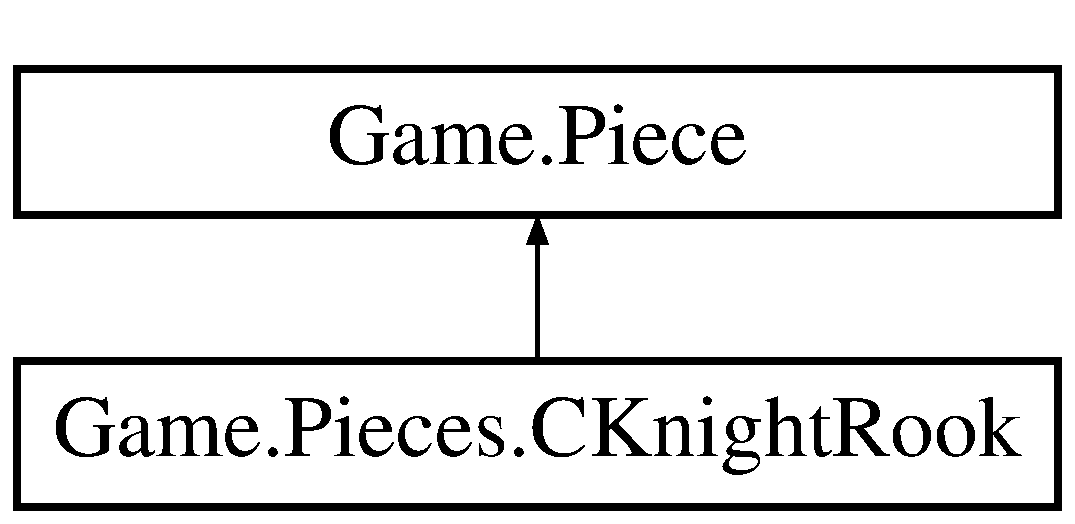
\includegraphics[height=2.000000cm]{class_game_1_1_pieces_1_1_c_knight_rook}
\end{center}
\end{figure}
\subsection*{Public Member Functions}
\begin{DoxyCompactItemize}
\item 
\hyperlink{class_game_1_1_pieces_1_1_c_knight_rook_ae86517971e5efa7e0ed0239a6138866b}{C\+Knight\+Rook} (int X, int Y, int c, \hyperlink{class_game_1_1_player}{Player} owner)
\item 
Array\+List$<$ \hyperlink{class_game_1_1_location}{Location} $>$ \hyperlink{class_game_1_1_pieces_1_1_c_knight_rook_addc2807f8d6c75a8e5bddcd098db5fb9}{explore\+\_\+possible\+\_\+positions} (\hyperlink{class_game_1_1_location}{Location} location, \hyperlink{class_game_1_1_chess_board}{Chess\+Board} chess\+Board)
\end{DoxyCompactItemize}
\subsection*{Additional Inherited Members}


\subsection{Constructor \& Destructor Documentation}
\mbox{\Hypertarget{class_game_1_1_pieces_1_1_c_knight_rook_ae86517971e5efa7e0ed0239a6138866b}\label{class_game_1_1_pieces_1_1_c_knight_rook_ae86517971e5efa7e0ed0239a6138866b}} 
\index{Game\+::\+Pieces\+::\+C\+Knight\+Rook@{Game\+::\+Pieces\+::\+C\+Knight\+Rook}!C\+Knight\+Rook@{C\+Knight\+Rook}}
\index{C\+Knight\+Rook@{C\+Knight\+Rook}!Game\+::\+Pieces\+::\+C\+Knight\+Rook@{Game\+::\+Pieces\+::\+C\+Knight\+Rook}}
\subsubsection{\texorpdfstring{C\+Knight\+Rook()}{CKnightRook()}}
{\footnotesize\ttfamily Game.\+Pieces.\+C\+Knight\+Rook.\+C\+Knight\+Rook (\begin{DoxyParamCaption}\item[{int}]{X,  }\item[{int}]{Y,  }\item[{int}]{c,  }\item[{\hyperlink{class_game_1_1_player}{Player}}]{owner }\end{DoxyParamCaption})\hspace{0.3cm}{\ttfamily [inline]}}

Constructor.


\begin{DoxyParams}{Parameters}
{\em c} & color of piece \\
\hline
{\em X} & X coordinate \\
\hline
{\em Y} & y coordinate \\
\hline
{\em owner} & is the owner of the piece \\
\hline
\end{DoxyParams}


\subsection{Member Function Documentation}
\mbox{\Hypertarget{class_game_1_1_pieces_1_1_c_knight_rook_addc2807f8d6c75a8e5bddcd098db5fb9}\label{class_game_1_1_pieces_1_1_c_knight_rook_addc2807f8d6c75a8e5bddcd098db5fb9}} 
\index{Game\+::\+Pieces\+::\+C\+Knight\+Rook@{Game\+::\+Pieces\+::\+C\+Knight\+Rook}!explore\+\_\+possible\+\_\+positions@{explore\+\_\+possible\+\_\+positions}}
\index{explore\+\_\+possible\+\_\+positions@{explore\+\_\+possible\+\_\+positions}!Game\+::\+Pieces\+::\+C\+Knight\+Rook@{Game\+::\+Pieces\+::\+C\+Knight\+Rook}}
\subsubsection{\texorpdfstring{explore\+\_\+possible\+\_\+positions()}{explore\_possible\_positions()}}
{\footnotesize\ttfamily Array\+List$<$\hyperlink{class_game_1_1_location}{Location}$>$ Game.\+Pieces.\+C\+Knight\+Rook.\+explore\+\_\+possible\+\_\+positions (\begin{DoxyParamCaption}\item[{\hyperlink{class_game_1_1_location}{Location}}]{location,  }\item[{\hyperlink{class_game_1_1_chess_board}{Chess\+Board}}]{chess\+Board }\end{DoxyParamCaption})\hspace{0.3cm}{\ttfamily [inline]}}

Explores all options for movement from location.


\begin{DoxyParams}{Parameters}
{\em location} & location from where we want to explore. \\
\hline
{\em chess\+Board} & is the chess board we are working on. \\
\hline
\end{DoxyParams}


The documentation for this class was generated from the following file\+:\begin{DoxyCompactItemize}
\item 
src/\+Game/\+Pieces/C\+Knight\+Rook.\+java\end{DoxyCompactItemize}

\hypertarget{class_tests_1_1_c_knight_rook_test}{}\section{Tests.\+C\+Knight\+Rook\+Test Class Reference}
\label{class_tests_1_1_c_knight_rook_test}\index{Tests.\+C\+Knight\+Rook\+Test@{Tests.\+C\+Knight\+Rook\+Test}}
\subsection*{Public Member Functions}
\begin{DoxyCompactItemize}
\item 
void \hyperlink{class_tests_1_1_c_knight_rook_test_aeaac63ecc2d7a359a7dbd50ccba581d0}{can\+Move\+To\+Cell\+Incorrect\+Test} ()  throws Exception 
\item 
void \hyperlink{class_tests_1_1_c_knight_rook_test_aaf2e223af58ebba13460dfd92892cff1}{can\+Move\+To\+Cell\+Correct\+Test} ()  throws Exception 
\item 
void \hyperlink{class_tests_1_1_c_knight_rook_test_a803bf9cf142b7ce8c59b8c500ce5e202}{explore\+\_\+possible\+\_\+positions\+All\+Test} ()  throws Exception 
\item 
void \hyperlink{class_tests_1_1_c_knight_rook_test_a3c50e04e4cb59f9cade207e7b79297d2}{explore\+\_\+possible\+\_\+positions\+Block\+Capture\+Test} ()  throws Exception 
\end{DoxyCompactItemize}


\subsection{Member Function Documentation}
\mbox{\Hypertarget{class_tests_1_1_c_knight_rook_test_aaf2e223af58ebba13460dfd92892cff1}\label{class_tests_1_1_c_knight_rook_test_aaf2e223af58ebba13460dfd92892cff1}} 
\index{Tests\+::\+C\+Knight\+Rook\+Test@{Tests\+::\+C\+Knight\+Rook\+Test}!can\+Move\+To\+Cell\+Correct\+Test@{can\+Move\+To\+Cell\+Correct\+Test}}
\index{can\+Move\+To\+Cell\+Correct\+Test@{can\+Move\+To\+Cell\+Correct\+Test}!Tests\+::\+C\+Knight\+Rook\+Test@{Tests\+::\+C\+Knight\+Rook\+Test}}
\subsubsection{\texorpdfstring{can\+Move\+To\+Cell\+Correct\+Test()}{canMoveToCellCorrectTest()}}
{\footnotesize\ttfamily void Tests.\+C\+Knight\+Rook\+Test.\+can\+Move\+To\+Cell\+Correct\+Test (\begin{DoxyParamCaption}{ }\end{DoxyParamCaption}) throws Exception\hspace{0.3cm}{\ttfamily [inline]}}

Check if King can move to correct piece. Should return true. \mbox{\Hypertarget{class_tests_1_1_c_knight_rook_test_aeaac63ecc2d7a359a7dbd50ccba581d0}\label{class_tests_1_1_c_knight_rook_test_aeaac63ecc2d7a359a7dbd50ccba581d0}} 
\index{Tests\+::\+C\+Knight\+Rook\+Test@{Tests\+::\+C\+Knight\+Rook\+Test}!can\+Move\+To\+Cell\+Incorrect\+Test@{can\+Move\+To\+Cell\+Incorrect\+Test}}
\index{can\+Move\+To\+Cell\+Incorrect\+Test@{can\+Move\+To\+Cell\+Incorrect\+Test}!Tests\+::\+C\+Knight\+Rook\+Test@{Tests\+::\+C\+Knight\+Rook\+Test}}
\subsubsection{\texorpdfstring{can\+Move\+To\+Cell\+Incorrect\+Test()}{canMoveToCellIncorrectTest()}}
{\footnotesize\ttfamily void Tests.\+C\+Knight\+Rook\+Test.\+can\+Move\+To\+Cell\+Incorrect\+Test (\begin{DoxyParamCaption}{ }\end{DoxyParamCaption}) throws Exception\hspace{0.3cm}{\ttfamily [inline]}}

Check if King can move to incorrect piece. Should return false. \mbox{\Hypertarget{class_tests_1_1_c_knight_rook_test_a803bf9cf142b7ce8c59b8c500ce5e202}\label{class_tests_1_1_c_knight_rook_test_a803bf9cf142b7ce8c59b8c500ce5e202}} 
\index{Tests\+::\+C\+Knight\+Rook\+Test@{Tests\+::\+C\+Knight\+Rook\+Test}!explore\+\_\+possible\+\_\+positions\+All\+Test@{explore\+\_\+possible\+\_\+positions\+All\+Test}}
\index{explore\+\_\+possible\+\_\+positions\+All\+Test@{explore\+\_\+possible\+\_\+positions\+All\+Test}!Tests\+::\+C\+Knight\+Rook\+Test@{Tests\+::\+C\+Knight\+Rook\+Test}}
\subsubsection{\texorpdfstring{explore\+\_\+possible\+\_\+positions\+All\+Test()}{explore\_possible\_positionsAllTest()}}
{\footnotesize\ttfamily void Tests.\+C\+Knight\+Rook\+Test.\+explore\+\_\+possible\+\_\+positions\+All\+Test (\begin{DoxyParamCaption}{ }\end{DoxyParamCaption}) throws Exception\hspace{0.3cm}{\ttfamily [inline]}}

Return all the places that a Rook can go from a position with no other pieces on board. \mbox{\Hypertarget{class_tests_1_1_c_knight_rook_test_a3c50e04e4cb59f9cade207e7b79297d2}\label{class_tests_1_1_c_knight_rook_test_a3c50e04e4cb59f9cade207e7b79297d2}} 
\index{Tests\+::\+C\+Knight\+Rook\+Test@{Tests\+::\+C\+Knight\+Rook\+Test}!explore\+\_\+possible\+\_\+positions\+Block\+Capture\+Test@{explore\+\_\+possible\+\_\+positions\+Block\+Capture\+Test}}
\index{explore\+\_\+possible\+\_\+positions\+Block\+Capture\+Test@{explore\+\_\+possible\+\_\+positions\+Block\+Capture\+Test}!Tests\+::\+C\+Knight\+Rook\+Test@{Tests\+::\+C\+Knight\+Rook\+Test}}
\subsubsection{\texorpdfstring{explore\+\_\+possible\+\_\+positions\+Block\+Capture\+Test()}{explore\_possible\_positionsBlockCaptureTest()}}
{\footnotesize\ttfamily void Tests.\+C\+Knight\+Rook\+Test.\+explore\+\_\+possible\+\_\+positions\+Block\+Capture\+Test (\begin{DoxyParamCaption}{ }\end{DoxyParamCaption}) throws Exception\hspace{0.3cm}{\ttfamily [inline]}}

Return all the places that a Rook can go from a position with some other pieces on board. 

The documentation for this class was generated from the following file\+:\begin{DoxyCompactItemize}
\item 
src/\+Tests/C\+Knight\+Rook\+Test.\+java\end{DoxyCompactItemize}

\hypertarget{class_game_1_1_pieces_1_1_king}{}\section{Game.\+Pieces.\+King Class Reference}
\label{class_game_1_1_pieces_1_1_king}\index{Game.\+Pieces.\+King@{Game.\+Pieces.\+King}}
Inheritance diagram for Game.\+Pieces.\+King\+:\begin{figure}[H]
\begin{center}
\leavevmode
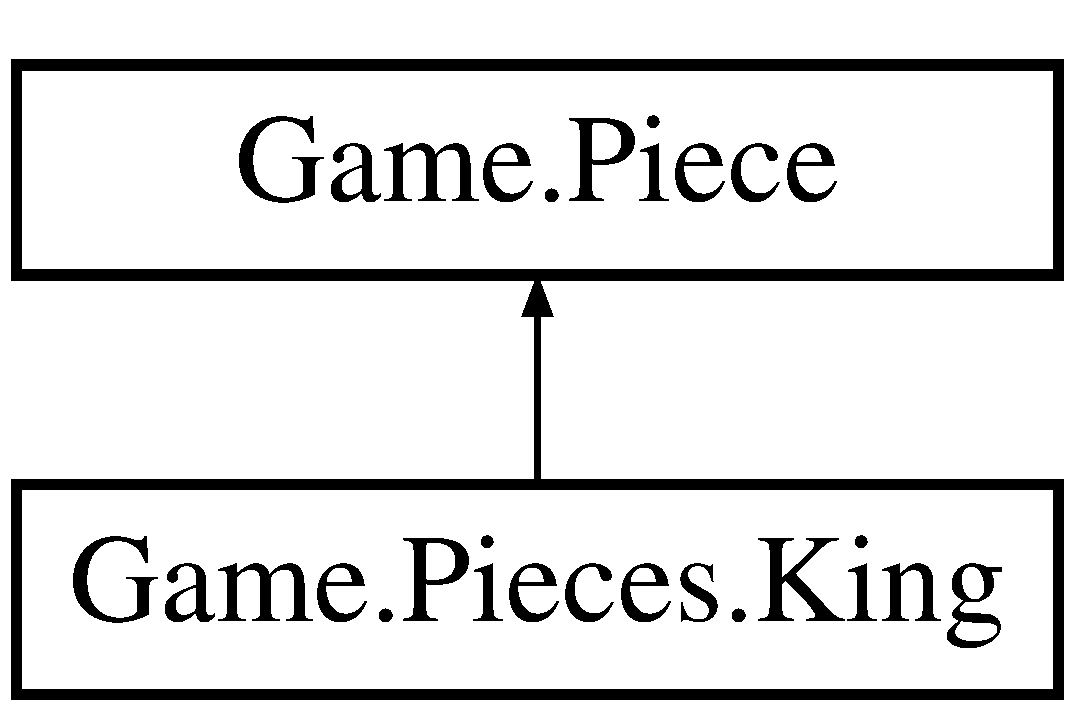
\includegraphics[height=2.000000cm]{class_game_1_1_pieces_1_1_king}
\end{center}
\end{figure}
\subsection*{Public Member Functions}
\begin{DoxyCompactItemize}
\item 
\hyperlink{class_game_1_1_pieces_1_1_king_abc8de10a53ab294f572e3554ba4e42bd}{King} (int X, int Y, int c, \hyperlink{class_game_1_1_player}{Player} owner)
\item 
Array\+List$<$ \hyperlink{class_game_1_1_location}{Location} $>$ \hyperlink{class_game_1_1_pieces_1_1_king_a15c52d6f4866a6a46f4b72b30b00636e}{explore\+\_\+possible\+\_\+positions} (\hyperlink{class_game_1_1_location}{Location} location, \hyperlink{class_game_1_1_chess_board}{Chess\+Board} chess\+Board)
\end{DoxyCompactItemize}
\subsection*{Additional Inherited Members}


\subsection{Constructor \& Destructor Documentation}
\mbox{\Hypertarget{class_game_1_1_pieces_1_1_king_abc8de10a53ab294f572e3554ba4e42bd}\label{class_game_1_1_pieces_1_1_king_abc8de10a53ab294f572e3554ba4e42bd}} 
\index{Game\+::\+Pieces\+::\+King@{Game\+::\+Pieces\+::\+King}!King@{King}}
\index{King@{King}!Game\+::\+Pieces\+::\+King@{Game\+::\+Pieces\+::\+King}}
\subsubsection{\texorpdfstring{King()}{King()}}
{\footnotesize\ttfamily Game.\+Pieces.\+King.\+King (\begin{DoxyParamCaption}\item[{int}]{X,  }\item[{int}]{Y,  }\item[{int}]{c,  }\item[{\hyperlink{class_game_1_1_player}{Player}}]{owner }\end{DoxyParamCaption})\hspace{0.3cm}{\ttfamily [inline]}}

Constructor. 
\begin{DoxyParams}{Parameters}
{\em c} & color of piece. \\
\hline
{\em X} & X coordinate. \\
\hline
{\em Y} & y coordinate. \\
\hline
{\em owner} & is the owner of the piece. \\
\hline
\end{DoxyParams}


\subsection{Member Function Documentation}
\mbox{\Hypertarget{class_game_1_1_pieces_1_1_king_a15c52d6f4866a6a46f4b72b30b00636e}\label{class_game_1_1_pieces_1_1_king_a15c52d6f4866a6a46f4b72b30b00636e}} 
\index{Game\+::\+Pieces\+::\+King@{Game\+::\+Pieces\+::\+King}!explore\+\_\+possible\+\_\+positions@{explore\+\_\+possible\+\_\+positions}}
\index{explore\+\_\+possible\+\_\+positions@{explore\+\_\+possible\+\_\+positions}!Game\+::\+Pieces\+::\+King@{Game\+::\+Pieces\+::\+King}}
\subsubsection{\texorpdfstring{explore\+\_\+possible\+\_\+positions()}{explore\_possible\_positions()}}
{\footnotesize\ttfamily Array\+List$<$\hyperlink{class_game_1_1_location}{Location}$>$ Game.\+Pieces.\+King.\+explore\+\_\+possible\+\_\+positions (\begin{DoxyParamCaption}\item[{\hyperlink{class_game_1_1_location}{Location}}]{location,  }\item[{\hyperlink{class_game_1_1_chess_board}{Chess\+Board}}]{chess\+Board }\end{DoxyParamCaption})\hspace{0.3cm}{\ttfamily [inline]}}

Explores all options for movement from location. 
\begin{DoxyParams}{Parameters}
{\em location} & location from where we want to explore. \\
\hline
{\em chess\+Board} & is the chess board we are working on. \\
\hline
\end{DoxyParams}


The documentation for this class was generated from the following file\+:\begin{DoxyCompactItemize}
\item 
src/\+Game/\+Pieces/King.\+java\end{DoxyCompactItemize}

\hypertarget{class_tests_1_1_king_test}{}\section{Tests.\+King\+Test Class Reference}
\label{class_tests_1_1_king_test}\index{Tests.\+King\+Test@{Tests.\+King\+Test}}
\subsection*{Public Member Functions}
\begin{DoxyCompactItemize}
\item 
void \hyperlink{class_tests_1_1_king_test_a734190e8769bb063e940021fe3aa4bd7}{can\+Move\+To\+Cell\+Incorrect\+Test} ()  throws Exception 
\item 
void \hyperlink{class_tests_1_1_king_test_aee8a0e677bbdd3f7de9967f3440986ca}{can\+Move\+To\+Cell\+Correct\+Test} ()  throws Exception 
\item 
void \hyperlink{class_tests_1_1_king_test_a9b38d5a81970a89bc5da02ecd10310c7}{explore\+\_\+possible\+\_\+positions\+All\+Test} ()  throws Exception 
\item 
void \hyperlink{class_tests_1_1_king_test_a83fff4dc942782651cdc9316b28b67da}{explore\+\_\+possible\+\_\+positions\+Blocked\+Capture\+Test} ()  throws Exception 
\end{DoxyCompactItemize}


\subsection{Member Function Documentation}
\mbox{\Hypertarget{class_tests_1_1_king_test_aee8a0e677bbdd3f7de9967f3440986ca}\label{class_tests_1_1_king_test_aee8a0e677bbdd3f7de9967f3440986ca}} 
\index{Tests\+::\+King\+Test@{Tests\+::\+King\+Test}!can\+Move\+To\+Cell\+Correct\+Test@{can\+Move\+To\+Cell\+Correct\+Test}}
\index{can\+Move\+To\+Cell\+Correct\+Test@{can\+Move\+To\+Cell\+Correct\+Test}!Tests\+::\+King\+Test@{Tests\+::\+King\+Test}}
\subsubsection{\texorpdfstring{can\+Move\+To\+Cell\+Correct\+Test()}{canMoveToCellCorrectTest()}}
{\footnotesize\ttfamily void Tests.\+King\+Test.\+can\+Move\+To\+Cell\+Correct\+Test (\begin{DoxyParamCaption}{ }\end{DoxyParamCaption}) throws Exception\hspace{0.3cm}{\ttfamily [inline]}}

Check if King can move to correct piece. Should return true. \mbox{\Hypertarget{class_tests_1_1_king_test_a734190e8769bb063e940021fe3aa4bd7}\label{class_tests_1_1_king_test_a734190e8769bb063e940021fe3aa4bd7}} 
\index{Tests\+::\+King\+Test@{Tests\+::\+King\+Test}!can\+Move\+To\+Cell\+Incorrect\+Test@{can\+Move\+To\+Cell\+Incorrect\+Test}}
\index{can\+Move\+To\+Cell\+Incorrect\+Test@{can\+Move\+To\+Cell\+Incorrect\+Test}!Tests\+::\+King\+Test@{Tests\+::\+King\+Test}}
\subsubsection{\texorpdfstring{can\+Move\+To\+Cell\+Incorrect\+Test()}{canMoveToCellIncorrectTest()}}
{\footnotesize\ttfamily void Tests.\+King\+Test.\+can\+Move\+To\+Cell\+Incorrect\+Test (\begin{DoxyParamCaption}{ }\end{DoxyParamCaption}) throws Exception\hspace{0.3cm}{\ttfamily [inline]}}

Check if King can move to wrong piece. Should return false. \mbox{\Hypertarget{class_tests_1_1_king_test_a9b38d5a81970a89bc5da02ecd10310c7}\label{class_tests_1_1_king_test_a9b38d5a81970a89bc5da02ecd10310c7}} 
\index{Tests\+::\+King\+Test@{Tests\+::\+King\+Test}!explore\+\_\+possible\+\_\+positions\+All\+Test@{explore\+\_\+possible\+\_\+positions\+All\+Test}}
\index{explore\+\_\+possible\+\_\+positions\+All\+Test@{explore\+\_\+possible\+\_\+positions\+All\+Test}!Tests\+::\+King\+Test@{Tests\+::\+King\+Test}}
\subsubsection{\texorpdfstring{explore\+\_\+possible\+\_\+positions\+All\+Test()}{explore\_possible\_positionsAllTest()}}
{\footnotesize\ttfamily void Tests.\+King\+Test.\+explore\+\_\+possible\+\_\+positions\+All\+Test (\begin{DoxyParamCaption}{ }\end{DoxyParamCaption}) throws Exception\hspace{0.3cm}{\ttfamily [inline]}}

Return all the places that a King can go from a position with no other pieces on board. \mbox{\Hypertarget{class_tests_1_1_king_test_a83fff4dc942782651cdc9316b28b67da}\label{class_tests_1_1_king_test_a83fff4dc942782651cdc9316b28b67da}} 
\index{Tests\+::\+King\+Test@{Tests\+::\+King\+Test}!explore\+\_\+possible\+\_\+positions\+Blocked\+Capture\+Test@{explore\+\_\+possible\+\_\+positions\+Blocked\+Capture\+Test}}
\index{explore\+\_\+possible\+\_\+positions\+Blocked\+Capture\+Test@{explore\+\_\+possible\+\_\+positions\+Blocked\+Capture\+Test}!Tests\+::\+King\+Test@{Tests\+::\+King\+Test}}
\subsubsection{\texorpdfstring{explore\+\_\+possible\+\_\+positions\+Blocked\+Capture\+Test()}{explore\_possible\_positionsBlockedCaptureTest()}}
{\footnotesize\ttfamily void Tests.\+King\+Test.\+explore\+\_\+possible\+\_\+positions\+Blocked\+Capture\+Test (\begin{DoxyParamCaption}{ }\end{DoxyParamCaption}) throws Exception\hspace{0.3cm}{\ttfamily [inline]}}

Return all the places that a King can go from a position with some other pieces on board. 

The documentation for this class was generated from the following file\+:\begin{DoxyCompactItemize}
\item 
src/\+Tests/King\+Test.\+java\end{DoxyCompactItemize}

\hypertarget{class_game_1_1_pieces_1_1_knight}{}\section{Game.\+Pieces.\+Knight Class Reference}
\label{class_game_1_1_pieces_1_1_knight}\index{Game.\+Pieces.\+Knight@{Game.\+Pieces.\+Knight}}
Inheritance diagram for Game.\+Pieces.\+Knight\+:\begin{figure}[H]
\begin{center}
\leavevmode
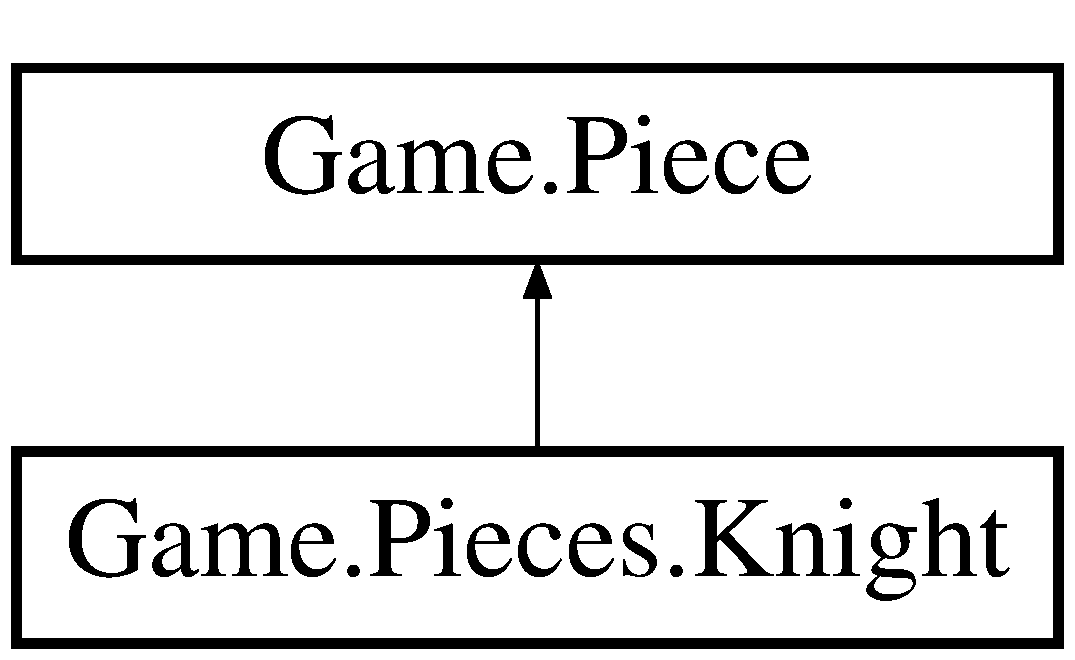
\includegraphics[height=2.000000cm]{class_game_1_1_pieces_1_1_knight}
\end{center}
\end{figure}
\subsection*{Public Member Functions}
\begin{DoxyCompactItemize}
\item 
\hyperlink{class_game_1_1_pieces_1_1_knight_af679624407663583c0f269ecd94ab4f9}{Knight} (int X, int Y, int c, \hyperlink{class_game_1_1_player}{Player} owner)
\item 
Array\+List$<$ \hyperlink{class_game_1_1_location}{Location} $>$ \hyperlink{class_game_1_1_pieces_1_1_knight_a0572a6b367275995dc4d9f8687595544}{explore\+\_\+possible\+\_\+positions} (\hyperlink{class_game_1_1_location}{Location} location, \hyperlink{class_game_1_1_chess_board}{Chess\+Board} chess\+Board)
\end{DoxyCompactItemize}
\subsection*{Additional Inherited Members}


\subsection{Constructor \& Destructor Documentation}
\mbox{\Hypertarget{class_game_1_1_pieces_1_1_knight_af679624407663583c0f269ecd94ab4f9}\label{class_game_1_1_pieces_1_1_knight_af679624407663583c0f269ecd94ab4f9}} 
\index{Game\+::\+Pieces\+::\+Knight@{Game\+::\+Pieces\+::\+Knight}!Knight@{Knight}}
\index{Knight@{Knight}!Game\+::\+Pieces\+::\+Knight@{Game\+::\+Pieces\+::\+Knight}}
\subsubsection{\texorpdfstring{Knight()}{Knight()}}
{\footnotesize\ttfamily Game.\+Pieces.\+Knight.\+Knight (\begin{DoxyParamCaption}\item[{int}]{X,  }\item[{int}]{Y,  }\item[{int}]{c,  }\item[{\hyperlink{class_game_1_1_player}{Player}}]{owner }\end{DoxyParamCaption})\hspace{0.3cm}{\ttfamily [inline]}}

Constructor. 
\begin{DoxyParams}{Parameters}
{\em c} & color of piece. \\
\hline
{\em X} & X coordinate. \\
\hline
{\em Y} & y coordinate. \\
\hline
{\em owner} & is the owner of the piece. \\
\hline
\end{DoxyParams}


\subsection{Member Function Documentation}
\mbox{\Hypertarget{class_game_1_1_pieces_1_1_knight_a0572a6b367275995dc4d9f8687595544}\label{class_game_1_1_pieces_1_1_knight_a0572a6b367275995dc4d9f8687595544}} 
\index{Game\+::\+Pieces\+::\+Knight@{Game\+::\+Pieces\+::\+Knight}!explore\+\_\+possible\+\_\+positions@{explore\+\_\+possible\+\_\+positions}}
\index{explore\+\_\+possible\+\_\+positions@{explore\+\_\+possible\+\_\+positions}!Game\+::\+Pieces\+::\+Knight@{Game\+::\+Pieces\+::\+Knight}}
\subsubsection{\texorpdfstring{explore\+\_\+possible\+\_\+positions()}{explore\_possible\_positions()}}
{\footnotesize\ttfamily Array\+List$<$\hyperlink{class_game_1_1_location}{Location}$>$ Game.\+Pieces.\+Knight.\+explore\+\_\+possible\+\_\+positions (\begin{DoxyParamCaption}\item[{\hyperlink{class_game_1_1_location}{Location}}]{location,  }\item[{\hyperlink{class_game_1_1_chess_board}{Chess\+Board}}]{chess\+Board }\end{DoxyParamCaption})\hspace{0.3cm}{\ttfamily [inline]}}

Explores all options for movement from location. 
\begin{DoxyParams}{Parameters}
{\em location} & location from where we want to explore. \\
\hline
{\em chess\+Board} & is the chess board we are working on. \\
\hline
\end{DoxyParams}


The documentation for this class was generated from the following file\+:\begin{DoxyCompactItemize}
\item 
src/\+Game/\+Pieces/Knight.\+java\end{DoxyCompactItemize}

\hypertarget{class_tests_1_1_knight_test}{}\section{Tests.\+Knight\+Test Class Reference}
\label{class_tests_1_1_knight_test}\index{Tests.\+Knight\+Test@{Tests.\+Knight\+Test}}
\subsection*{Public Member Functions}
\begin{DoxyCompactItemize}
\item 
void \hyperlink{class_tests_1_1_knight_test_a2a0d937a0083e7713c0dd50c7dac26de}{can\+Move\+To\+Cell\+Incorrect\+Test} ()  throws Exception 
\item 
void \hyperlink{class_tests_1_1_knight_test_a4ba3c282719c171123c4befad34ff86a}{can\+Move\+To\+Cell\+Correct\+Test} ()  throws Exception 
\item 
void \hyperlink{class_tests_1_1_knight_test_a870d8cf9b905eafc3f24d34c2e83b163}{explore\+\_\+possible\+\_\+positions\+All\+Test} ()  throws Exception 
\item 
void \hyperlink{class_tests_1_1_knight_test_ab48152da0c4686a6baadc268e313ca54}{explore\+\_\+possible\+\_\+positions\+Block\+Capture\+Test} ()  throws Exception 
\end{DoxyCompactItemize}


\subsection{Member Function Documentation}
\mbox{\Hypertarget{class_tests_1_1_knight_test_a4ba3c282719c171123c4befad34ff86a}\label{class_tests_1_1_knight_test_a4ba3c282719c171123c4befad34ff86a}} 
\index{Tests\+::\+Knight\+Test@{Tests\+::\+Knight\+Test}!can\+Move\+To\+Cell\+Correct\+Test@{can\+Move\+To\+Cell\+Correct\+Test}}
\index{can\+Move\+To\+Cell\+Correct\+Test@{can\+Move\+To\+Cell\+Correct\+Test}!Tests\+::\+Knight\+Test@{Tests\+::\+Knight\+Test}}
\subsubsection{\texorpdfstring{can\+Move\+To\+Cell\+Correct\+Test()}{canMoveToCellCorrectTest()}}
{\footnotesize\ttfamily void Tests.\+Knight\+Test.\+can\+Move\+To\+Cell\+Correct\+Test (\begin{DoxyParamCaption}{ }\end{DoxyParamCaption}) throws Exception\hspace{0.3cm}{\ttfamily [inline]}}

Check if King can move to correct piece. Should return true. \mbox{\Hypertarget{class_tests_1_1_knight_test_a2a0d937a0083e7713c0dd50c7dac26de}\label{class_tests_1_1_knight_test_a2a0d937a0083e7713c0dd50c7dac26de}} 
\index{Tests\+::\+Knight\+Test@{Tests\+::\+Knight\+Test}!can\+Move\+To\+Cell\+Incorrect\+Test@{can\+Move\+To\+Cell\+Incorrect\+Test}}
\index{can\+Move\+To\+Cell\+Incorrect\+Test@{can\+Move\+To\+Cell\+Incorrect\+Test}!Tests\+::\+Knight\+Test@{Tests\+::\+Knight\+Test}}
\subsubsection{\texorpdfstring{can\+Move\+To\+Cell\+Incorrect\+Test()}{canMoveToCellIncorrectTest()}}
{\footnotesize\ttfamily void Tests.\+Knight\+Test.\+can\+Move\+To\+Cell\+Incorrect\+Test (\begin{DoxyParamCaption}{ }\end{DoxyParamCaption}) throws Exception\hspace{0.3cm}{\ttfamily [inline]}}

Check if King can move to incorrect piece. Should return false. \mbox{\Hypertarget{class_tests_1_1_knight_test_a870d8cf9b905eafc3f24d34c2e83b163}\label{class_tests_1_1_knight_test_a870d8cf9b905eafc3f24d34c2e83b163}} 
\index{Tests\+::\+Knight\+Test@{Tests\+::\+Knight\+Test}!explore\+\_\+possible\+\_\+positions\+All\+Test@{explore\+\_\+possible\+\_\+positions\+All\+Test}}
\index{explore\+\_\+possible\+\_\+positions\+All\+Test@{explore\+\_\+possible\+\_\+positions\+All\+Test}!Tests\+::\+Knight\+Test@{Tests\+::\+Knight\+Test}}
\subsubsection{\texorpdfstring{explore\+\_\+possible\+\_\+positions\+All\+Test()}{explore\_possible\_positionsAllTest()}}
{\footnotesize\ttfamily void Tests.\+Knight\+Test.\+explore\+\_\+possible\+\_\+positions\+All\+Test (\begin{DoxyParamCaption}{ }\end{DoxyParamCaption}) throws Exception\hspace{0.3cm}{\ttfamily [inline]}}

Return all the places that a Knight can go from a position with no other pieces on board. \mbox{\Hypertarget{class_tests_1_1_knight_test_ab48152da0c4686a6baadc268e313ca54}\label{class_tests_1_1_knight_test_ab48152da0c4686a6baadc268e313ca54}} 
\index{Tests\+::\+Knight\+Test@{Tests\+::\+Knight\+Test}!explore\+\_\+possible\+\_\+positions\+Block\+Capture\+Test@{explore\+\_\+possible\+\_\+positions\+Block\+Capture\+Test}}
\index{explore\+\_\+possible\+\_\+positions\+Block\+Capture\+Test@{explore\+\_\+possible\+\_\+positions\+Block\+Capture\+Test}!Tests\+::\+Knight\+Test@{Tests\+::\+Knight\+Test}}
\subsubsection{\texorpdfstring{explore\+\_\+possible\+\_\+positions\+Block\+Capture\+Test()}{explore\_possible\_positionsBlockCaptureTest()}}
{\footnotesize\ttfamily void Tests.\+Knight\+Test.\+explore\+\_\+possible\+\_\+positions\+Block\+Capture\+Test (\begin{DoxyParamCaption}{ }\end{DoxyParamCaption}) throws Exception\hspace{0.3cm}{\ttfamily [inline]}}

Return all the places that a Knight can go from a position with some other pieces on board. 

The documentation for this class was generated from the following file\+:\begin{DoxyCompactItemize}
\item 
src/\+Tests/Knight\+Test.\+java\end{DoxyCompactItemize}

\hypertarget{class_game_1_1_location}{}\section{Game.\+Location Class Reference}
\label{class_game_1_1_location}\index{Game.\+Location@{Game.\+Location}}
\subsection*{Public Member Functions}
\begin{DoxyCompactItemize}
\item 
\hyperlink{class_game_1_1_location_a2495e651aa5fd0e0ceadd214110c7636}{Location} (int X, int Y)
\item 
\mbox{\Hypertarget{class_game_1_1_location_a885d1e5e9db3fa1952bd19d3c16cd692}\label{class_game_1_1_location_a885d1e5e9db3fa1952bd19d3c16cd692}} 
void {\bfseries print\+Loc} ()
\item 
\mbox{\Hypertarget{class_game_1_1_location_a05a33b631edc58aca142cbfd764cf959}\label{class_game_1_1_location_a05a33b631edc58aca142cbfd764cf959}} 
int {\bfseries get\+Rank} ()
\item 
\mbox{\Hypertarget{class_game_1_1_location_ac1b54da6df376f41b06b53307e5cf42f}\label{class_game_1_1_location_ac1b54da6df376f41b06b53307e5cf42f}} 
int {\bfseries get\+File} ()
\item 
\mbox{\Hypertarget{class_game_1_1_location_ab714802f95d86395573a9fb6533da284}\label{class_game_1_1_location_ab714802f95d86395573a9fb6533da284}} 
String {\bfseries get\+\_\+location\+\_\+name} ()
\item 
\mbox{\Hypertarget{class_game_1_1_location_a199a32db7abcccfd986bb4477f67aa12}\label{class_game_1_1_location_a199a32db7abcccfd986bb4477f67aa12}} 
boolean {\bfseries is\+On\+Board} ()
\end{DoxyCompactItemize}


\subsection{Constructor \& Destructor Documentation}
\mbox{\Hypertarget{class_game_1_1_location_a2495e651aa5fd0e0ceadd214110c7636}\label{class_game_1_1_location_a2495e651aa5fd0e0ceadd214110c7636}} 
\index{Game\+::\+Location@{Game\+::\+Location}!Location@{Location}}
\index{Location@{Location}!Game\+::\+Location@{Game\+::\+Location}}
\subsubsection{\texorpdfstring{Location()}{Location()}}
{\footnotesize\ttfamily Game.\+Location.\+Location (\begin{DoxyParamCaption}\item[{int}]{X,  }\item[{int}]{Y }\end{DoxyParamCaption})\hspace{0.3cm}{\ttfamily [inline]}}

This class contains the llocations of each piece. It has an x coordinate. It has a y coordinate. And a string name 

The documentation for this class was generated from the following file\+:\begin{DoxyCompactItemize}
\item 
src/\+Game/Location.\+java\end{DoxyCompactItemize}

\hypertarget{class_game_1_1_pieces_1_1_pawn}{}\section{Game.\+Pieces.\+Pawn Class Reference}
\label{class_game_1_1_pieces_1_1_pawn}\index{Game.\+Pieces.\+Pawn@{Game.\+Pieces.\+Pawn}}
Inheritance diagram for Game.\+Pieces.\+Pawn\+:\begin{figure}[H]
\begin{center}
\leavevmode
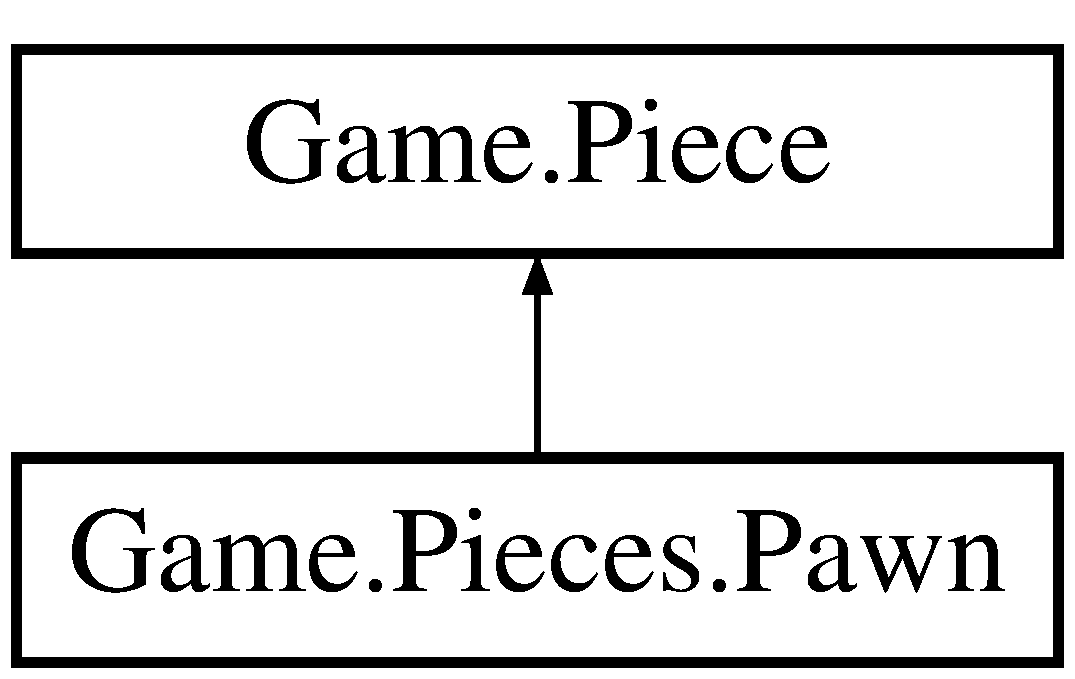
\includegraphics[height=2.000000cm]{class_game_1_1_pieces_1_1_pawn}
\end{center}
\end{figure}
\subsection*{Public Member Functions}
\begin{DoxyCompactItemize}
\item 
\hyperlink{class_game_1_1_pieces_1_1_pawn_aaa1f423adede7444520459ea607f0f36}{Pawn} (int X, int Y, int c, \hyperlink{class_game_1_1_player}{Player} owner)
\item 
Array\+List$<$ \hyperlink{class_game_1_1_location}{Location} $>$ \hyperlink{class_game_1_1_pieces_1_1_pawn_ae017bf02eaa2725e81b3e090570621ce}{explore\+\_\+possible\+\_\+positions} (\hyperlink{class_game_1_1_location}{Location} location, \hyperlink{class_game_1_1_chess_board}{Chess\+Board} chess\+Board)
\item 
int \mbox{[}$\,$\mbox{]}\mbox{[}$\,$\mbox{]} \hyperlink{class_game_1_1_pieces_1_1_pawn_adf35b286f0743f944785fc916cdea79b}{move} (\hyperlink{class_game_1_1_location}{Location} location, \hyperlink{class_game_1_1_location}{Location} destination, \hyperlink{class_game_1_1_chess_board}{Chess\+Board} chess\+Board)
\end{DoxyCompactItemize}
\subsection*{Additional Inherited Members}


\subsection{Constructor \& Destructor Documentation}
\mbox{\Hypertarget{class_game_1_1_pieces_1_1_pawn_aaa1f423adede7444520459ea607f0f36}\label{class_game_1_1_pieces_1_1_pawn_aaa1f423adede7444520459ea607f0f36}} 
\index{Game\+::\+Pieces\+::\+Pawn@{Game\+::\+Pieces\+::\+Pawn}!Pawn@{Pawn}}
\index{Pawn@{Pawn}!Game\+::\+Pieces\+::\+Pawn@{Game\+::\+Pieces\+::\+Pawn}}
\subsubsection{\texorpdfstring{Pawn()}{Pawn()}}
{\footnotesize\ttfamily Game.\+Pieces.\+Pawn.\+Pawn (\begin{DoxyParamCaption}\item[{int}]{X,  }\item[{int}]{Y,  }\item[{int}]{c,  }\item[{\hyperlink{class_game_1_1_player}{Player}}]{owner }\end{DoxyParamCaption})\hspace{0.3cm}{\ttfamily [inline]}}

Constructor. 
\begin{DoxyParams}{Parameters}
{\em c} & color of piece. \\
\hline
{\em X} & X coordinate. \\
\hline
{\em Y} & y coordinate. \\
\hline
{\em owner} & is the owner of the piece. \\
\hline
\end{DoxyParams}


\subsection{Member Function Documentation}
\mbox{\Hypertarget{class_game_1_1_pieces_1_1_pawn_ae017bf02eaa2725e81b3e090570621ce}\label{class_game_1_1_pieces_1_1_pawn_ae017bf02eaa2725e81b3e090570621ce}} 
\index{Game\+::\+Pieces\+::\+Pawn@{Game\+::\+Pieces\+::\+Pawn}!explore\+\_\+possible\+\_\+positions@{explore\+\_\+possible\+\_\+positions}}
\index{explore\+\_\+possible\+\_\+positions@{explore\+\_\+possible\+\_\+positions}!Game\+::\+Pieces\+::\+Pawn@{Game\+::\+Pieces\+::\+Pawn}}
\subsubsection{\texorpdfstring{explore\+\_\+possible\+\_\+positions()}{explore\_possible\_positions()}}
{\footnotesize\ttfamily Array\+List$<$\hyperlink{class_game_1_1_location}{Location}$>$ Game.\+Pieces.\+Pawn.\+explore\+\_\+possible\+\_\+positions (\begin{DoxyParamCaption}\item[{\hyperlink{class_game_1_1_location}{Location}}]{location,  }\item[{\hyperlink{class_game_1_1_chess_board}{Chess\+Board}}]{chess\+Board }\end{DoxyParamCaption})\hspace{0.3cm}{\ttfamily [inline]}}

Explores all options for movement from location. 
\begin{DoxyParams}{Parameters}
{\em location} & location from where we want to explore. \\
\hline
{\em chess\+Board} & is the chess board we are working on. \\
\hline
\end{DoxyParams}
\mbox{\Hypertarget{class_game_1_1_pieces_1_1_pawn_adf35b286f0743f944785fc916cdea79b}\label{class_game_1_1_pieces_1_1_pawn_adf35b286f0743f944785fc916cdea79b}} 
\index{Game\+::\+Pieces\+::\+Pawn@{Game\+::\+Pieces\+::\+Pawn}!move@{move}}
\index{move@{move}!Game\+::\+Pieces\+::\+Pawn@{Game\+::\+Pieces\+::\+Pawn}}
\subsubsection{\texorpdfstring{move()}{move()}}
{\footnotesize\ttfamily int \mbox{[}$\,$\mbox{]}\mbox{[}$\,$\mbox{]} Game.\+Pieces.\+Pawn.\+move (\begin{DoxyParamCaption}\item[{\hyperlink{class_game_1_1_location}{Location}}]{location,  }\item[{\hyperlink{class_game_1_1_location}{Location}}]{destination,  }\item[{\hyperlink{class_game_1_1_chess_board}{Chess\+Board}}]{chess\+Board }\end{DoxyParamCaption})\hspace{0.3cm}{\ttfamily [inline]}}

Move to destination and then set first turn to false. 
\begin{DoxyParams}{Parameters}
{\em location} & location from where we want to leave. \\
\hline
{\em destination} & location we want to reach. \\
\hline
{\em chess\+Board} & is the chess board we are working on. \\
\hline
\end{DoxyParams}


The documentation for this class was generated from the following file\+:\begin{DoxyCompactItemize}
\item 
src/\+Game/\+Pieces/Pawn.\+java\end{DoxyCompactItemize}

\hypertarget{class_tests_1_1_pawn_test}{}\section{Tests.\+Pawn\+Test Class Reference}
\label{class_tests_1_1_pawn_test}\index{Tests.\+Pawn\+Test@{Tests.\+Pawn\+Test}}
\subsection*{Public Member Functions}
\begin{DoxyCompactItemize}
\item 
void \hyperlink{class_tests_1_1_pawn_test_aec96d9b7e52313d9da19774d4f5eb930}{can\+Move\+To\+Cell\+Incorrect\+Test} ()  throws Exception 
\item 
void \hyperlink{class_tests_1_1_pawn_test_a0c6b158dbc92e9ec87469953766229bd}{can\+Move\+To\+Cell\+Correct\+Test} ()  throws Exception 
\item 
void \hyperlink{class_tests_1_1_pawn_test_a668f1c8e1e03f1d7f3c57c52881e1246}{explore\+\_\+possible\+\_\+positions\+All\+Test} ()  throws Exception 
\item 
void \hyperlink{class_tests_1_1_pawn_test_acc141a39019b36025a8a3aad46c00968}{explore\+\_\+possible\+\_\+positions\+Block\+Capture\+Test} ()  throws Exception 
\end{DoxyCompactItemize}


\subsection{Member Function Documentation}
\mbox{\Hypertarget{class_tests_1_1_pawn_test_a0c6b158dbc92e9ec87469953766229bd}\label{class_tests_1_1_pawn_test_a0c6b158dbc92e9ec87469953766229bd}} 
\index{Tests\+::\+Pawn\+Test@{Tests\+::\+Pawn\+Test}!can\+Move\+To\+Cell\+Correct\+Test@{can\+Move\+To\+Cell\+Correct\+Test}}
\index{can\+Move\+To\+Cell\+Correct\+Test@{can\+Move\+To\+Cell\+Correct\+Test}!Tests\+::\+Pawn\+Test@{Tests\+::\+Pawn\+Test}}
\subsubsection{\texorpdfstring{can\+Move\+To\+Cell\+Correct\+Test()}{canMoveToCellCorrectTest()}}
{\footnotesize\ttfamily void Tests.\+Pawn\+Test.\+can\+Move\+To\+Cell\+Correct\+Test (\begin{DoxyParamCaption}{ }\end{DoxyParamCaption}) throws Exception\hspace{0.3cm}{\ttfamily [inline]}}

Check if King can move to incorrect piece. Should return false. \mbox{\Hypertarget{class_tests_1_1_pawn_test_aec96d9b7e52313d9da19774d4f5eb930}\label{class_tests_1_1_pawn_test_aec96d9b7e52313d9da19774d4f5eb930}} 
\index{Tests\+::\+Pawn\+Test@{Tests\+::\+Pawn\+Test}!can\+Move\+To\+Cell\+Incorrect\+Test@{can\+Move\+To\+Cell\+Incorrect\+Test}}
\index{can\+Move\+To\+Cell\+Incorrect\+Test@{can\+Move\+To\+Cell\+Incorrect\+Test}!Tests\+::\+Pawn\+Test@{Tests\+::\+Pawn\+Test}}
\subsubsection{\texorpdfstring{can\+Move\+To\+Cell\+Incorrect\+Test()}{canMoveToCellIncorrectTest()}}
{\footnotesize\ttfamily void Tests.\+Pawn\+Test.\+can\+Move\+To\+Cell\+Incorrect\+Test (\begin{DoxyParamCaption}{ }\end{DoxyParamCaption}) throws Exception\hspace{0.3cm}{\ttfamily [inline]}}

Check if King can move to incorrect piece. Should return false. \mbox{\Hypertarget{class_tests_1_1_pawn_test_a668f1c8e1e03f1d7f3c57c52881e1246}\label{class_tests_1_1_pawn_test_a668f1c8e1e03f1d7f3c57c52881e1246}} 
\index{Tests\+::\+Pawn\+Test@{Tests\+::\+Pawn\+Test}!explore\+\_\+possible\+\_\+positions\+All\+Test@{explore\+\_\+possible\+\_\+positions\+All\+Test}}
\index{explore\+\_\+possible\+\_\+positions\+All\+Test@{explore\+\_\+possible\+\_\+positions\+All\+Test}!Tests\+::\+Pawn\+Test@{Tests\+::\+Pawn\+Test}}
\subsubsection{\texorpdfstring{explore\+\_\+possible\+\_\+positions\+All\+Test()}{explore\_possible\_positionsAllTest()}}
{\footnotesize\ttfamily void Tests.\+Pawn\+Test.\+explore\+\_\+possible\+\_\+positions\+All\+Test (\begin{DoxyParamCaption}{ }\end{DoxyParamCaption}) throws Exception\hspace{0.3cm}{\ttfamily [inline]}}

Return all the places that a Pawn can go from a position with no other pieces on board. \mbox{\Hypertarget{class_tests_1_1_pawn_test_acc141a39019b36025a8a3aad46c00968}\label{class_tests_1_1_pawn_test_acc141a39019b36025a8a3aad46c00968}} 
\index{Tests\+::\+Pawn\+Test@{Tests\+::\+Pawn\+Test}!explore\+\_\+possible\+\_\+positions\+Block\+Capture\+Test@{explore\+\_\+possible\+\_\+positions\+Block\+Capture\+Test}}
\index{explore\+\_\+possible\+\_\+positions\+Block\+Capture\+Test@{explore\+\_\+possible\+\_\+positions\+Block\+Capture\+Test}!Tests\+::\+Pawn\+Test@{Tests\+::\+Pawn\+Test}}
\subsubsection{\texorpdfstring{explore\+\_\+possible\+\_\+positions\+Block\+Capture\+Test()}{explore\_possible\_positionsBlockCaptureTest()}}
{\footnotesize\ttfamily void Tests.\+Pawn\+Test.\+explore\+\_\+possible\+\_\+positions\+Block\+Capture\+Test (\begin{DoxyParamCaption}{ }\end{DoxyParamCaption}) throws Exception\hspace{0.3cm}{\ttfamily [inline]}}

Return all the places that a Pawn can go from a position with some other pieces on board. 

The documentation for this class was generated from the following file\+:\begin{DoxyCompactItemize}
\item 
src/\+Tests/Pawn\+Test.\+java\end{DoxyCompactItemize}

\hypertarget{class_game_1_1_piece}{}\section{Game.\+Piece Class Reference}
\label{class_game_1_1_piece}\index{Game.\+Piece@{Game.\+Piece}}
Inheritance diagram for Game.\+Piece\+:\begin{figure}[H]
\begin{center}
\leavevmode
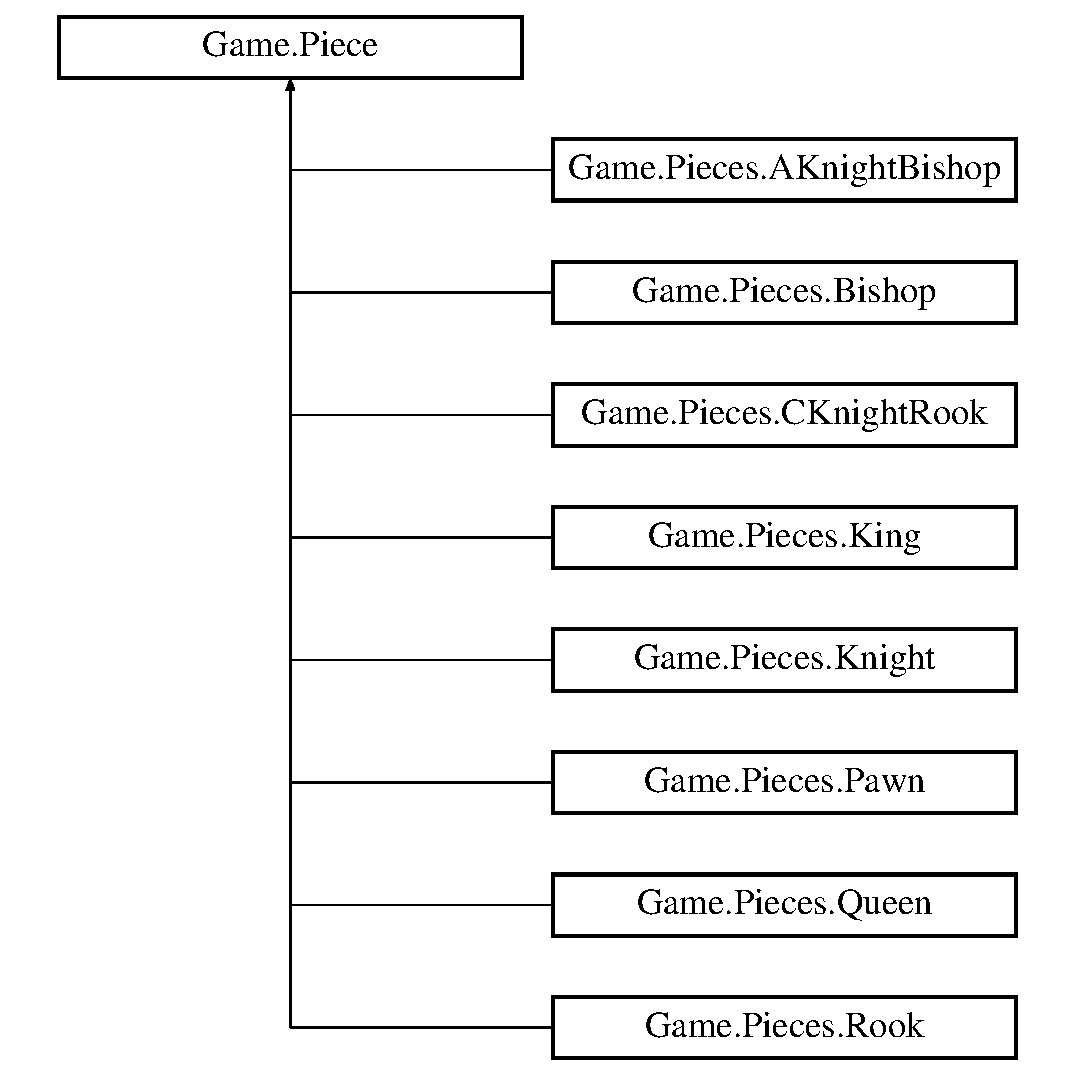
\includegraphics[height=9.000000cm]{class_game_1_1_piece}
\end{center}
\end{figure}
\subsection*{Public Member Functions}
\begin{DoxyCompactItemize}
\item 
\hyperlink{class_game_1_1_piece_ac7bf4a99bb03a745e9b857c8091c3304}{Piece} ()
\item 
boolean \hyperlink{class_game_1_1_piece_a731841b5bb47df461d9de450386e937b}{is\+Out\+Board} (\hyperlink{class_game_1_1_location}{Location} location)
\item 
\mbox{\Hypertarget{class_game_1_1_piece_af5a0f0900601ca2ba564c58f528e3e1f}\label{class_game_1_1_piece_af5a0f0900601ca2ba564c58f528e3e1f}} 
Array\+List$<$ \hyperlink{class_game_1_1_location}{Location} $>$ {\bfseries explore\+\_\+possible\+\_\+positions} (\hyperlink{class_game_1_1_location}{Location} location, \hyperlink{class_game_1_1_chess_board}{Chess\+Board} chess\+Board)
\item 
\mbox{\Hypertarget{class_game_1_1_piece_a944c18376b6af8bd8d695867a1cb7ea6}\label{class_game_1_1_piece_a944c18376b6af8bd8d695867a1cb7ea6}} 
\hyperlink{class_game_1_1_location}{Location} {\bfseries get\+\_\+location} ()
\item 
\mbox{\Hypertarget{class_game_1_1_piece_a2bc8c96480246808852708360cad25a1}\label{class_game_1_1_piece_a2bc8c96480246808852708360cad25a1}} 
String {\bfseries get\+\_\+name} ()
\item 
\mbox{\Hypertarget{class_game_1_1_piece_ac7d27da23e3311567b6e773c7da17da0}\label{class_game_1_1_piece_ac7d27da23e3311567b6e773c7da17da0}} 
int {\bfseries get\+Color} ()
\item 
\mbox{\Hypertarget{class_game_1_1_piece_ac1da8a79281f3cd6fea02044c47a5b03}\label{class_game_1_1_piece_ac1da8a79281f3cd6fea02044c47a5b03}} 
int {\bfseries get\+Value} ()
\item 
\mbox{\Hypertarget{class_game_1_1_piece_a5a0fcd7f275b131d76312dd58d851dee}\label{class_game_1_1_piece_a5a0fcd7f275b131d76312dd58d851dee}} 
\hyperlink{class_game_1_1_player}{Player} {\bfseries get\+\_\+owner} ()
\item 
int \mbox{[}$\,$\mbox{]}\mbox{[}$\,$\mbox{]} \hyperlink{class_game_1_1_piece_a1edfb33b56e00ac858f1dfe34739c19e}{move} (\hyperlink{class_game_1_1_location}{Location} location, \hyperlink{class_game_1_1_location}{Location} destination, \hyperlink{class_game_1_1_chess_board}{Chess\+Board} chess\+Board)
\item 
\mbox{\Hypertarget{class_game_1_1_piece_ab66d90e85bab97d03ddba72d3736ae27}\label{class_game_1_1_piece_ab66d90e85bab97d03ddba72d3736ae27}} 
boolean {\bfseries can\+Capture} (\hyperlink{class_game_1_1_location}{Location} location, \hyperlink{class_game_1_1_location}{Location} destination, Hash\+Map$<$ \hyperlink{class_game_1_1_location}{Location}, \hyperlink{class_game_1_1_piece}{Piece} $>$ board)
\item 
\mbox{\Hypertarget{class_game_1_1_piece_ac436d4c58f325d6ce7ab1000098a00d1}\label{class_game_1_1_piece_ac436d4c58f325d6ce7ab1000098a00d1}} 
boolean {\bfseries position\+Occupied} (\hyperlink{class_game_1_1_location}{Location} loc, Hash\+Map$<$ \hyperlink{class_game_1_1_location}{Location}, \hyperlink{class_game_1_1_piece}{Piece} $>$ board)
\item 
int \mbox{[}$\,$\mbox{]}\mbox{[}$\,$\mbox{]} \hyperlink{class_game_1_1_piece_acc0658b488de0531c94899ff16f81860}{undo\+Move} (\hyperlink{class_game_1_1_location}{Location} location, \hyperlink{class_game_1_1_location}{Location} destination, \hyperlink{class_game_1_1_piece}{Piece} captured\+Piece, \hyperlink{class_game_1_1_chess_board}{Chess\+Board} chess\+Board)
\item 
boolean \hyperlink{class_game_1_1_piece_a8db59115b31d53cfb6e8b31df38f22ab}{can\+Move\+To} (\hyperlink{class_game_1_1_location}{Location} location, \hyperlink{class_game_1_1_location}{Location} destination, \hyperlink{class_game_1_1_chess_board}{Chess\+Board} chess\+Board)
\end{DoxyCompactItemize}
\subsection*{Protected Member Functions}
\begin{DoxyCompactItemize}
\item 
void \hyperlink{class_game_1_1_piece_a693ab25eaea3b524fc34ddd0da52576e}{add\+Moves\+In\+Line} (\hyperlink{class_game_1_1_location}{Location} location, \hyperlink{class_game_1_1_chess_board}{Chess\+Board} chess\+Board, Array\+List$<$ \hyperlink{class_game_1_1_location}{Location} $>$ moves, int xi, int yi)
\item 
void \hyperlink{class_game_1_1_piece_a66a1001c4c88e92b73575c332c29b01e}{add\+If\+Valid} (\hyperlink{class_game_1_1_location}{Location} location, \hyperlink{class_game_1_1_chess_board}{Chess\+Board} chess\+Board, Array\+List$<$ \hyperlink{class_game_1_1_location}{Location} $>$ moves, int xi, int yi)
\end{DoxyCompactItemize}
\subsection*{Protected Attributes}
\begin{DoxyCompactItemize}
\item 
\mbox{\Hypertarget{class_game_1_1_piece_a75996931e37b3a17b2638dfa374fd47b}\label{class_game_1_1_piece_a75996931e37b3a17b2638dfa374fd47b}} 
\hyperlink{class_game_1_1_player}{Player} {\bfseries owner}
\item 
\mbox{\Hypertarget{class_game_1_1_piece_a68b7c8cc66bcc4d5e5f44fb300892986}\label{class_game_1_1_piece_a68b7c8cc66bcc4d5e5f44fb300892986}} 
int {\bfseries color}
\item 
\mbox{\Hypertarget{class_game_1_1_piece_a28af46d97aaf22e65132802600c036eb}\label{class_game_1_1_piece_a28af46d97aaf22e65132802600c036eb}} 
int {\bfseries value} = 0
\item 
\mbox{\Hypertarget{class_game_1_1_piece_aed829bf40fb2e53850e907721ea9614e}\label{class_game_1_1_piece_aed829bf40fb2e53850e907721ea9614e}} 
String {\bfseries kind}
\item 
\mbox{\Hypertarget{class_game_1_1_piece_a757648998fb60105600446e82ffdc711}\label{class_game_1_1_piece_a757648998fb60105600446e82ffdc711}} 
Array\+List$<$ \hyperlink{class_game_1_1_location}{Location} $>$ {\bfseries possible\+\_\+positions}
\item 
\mbox{\Hypertarget{class_game_1_1_piece_a3cc8f2b3246e0a8c2801c3215f30ff1c}\label{class_game_1_1_piece_a3cc8f2b3246e0a8c2801c3215f30ff1c}} 
boolean {\bfseries can\+\_\+move}
\item 
\mbox{\Hypertarget{class_game_1_1_piece_ae34b20097d771631ff6bff635d2fde3d}\label{class_game_1_1_piece_ae34b20097d771631ff6bff635d2fde3d}} 
\hyperlink{class_game_1_1_location}{Location} {\bfseries location}
\end{DoxyCompactItemize}


\subsection{Constructor \& Destructor Documentation}
\mbox{\Hypertarget{class_game_1_1_piece_ac7bf4a99bb03a745e9b857c8091c3304}\label{class_game_1_1_piece_ac7bf4a99bb03a745e9b857c8091c3304}} 
\index{Game\+::\+Piece@{Game\+::\+Piece}!Piece@{Piece}}
\index{Piece@{Piece}!Game\+::\+Piece@{Game\+::\+Piece}}
\subsubsection{\texorpdfstring{Piece()}{Piece()}}
{\footnotesize\ttfamily Game.\+Piece.\+Piece (\begin{DoxyParamCaption}{ }\end{DoxyParamCaption})\hspace{0.3cm}{\ttfamily [inline]}}

Constructor for piece, returns an empty piece which can be replaced. 

\subsection{Member Function Documentation}
\mbox{\Hypertarget{class_game_1_1_piece_a66a1001c4c88e92b73575c332c29b01e}\label{class_game_1_1_piece_a66a1001c4c88e92b73575c332c29b01e}} 
\index{Game\+::\+Piece@{Game\+::\+Piece}!add\+If\+Valid@{add\+If\+Valid}}
\index{add\+If\+Valid@{add\+If\+Valid}!Game\+::\+Piece@{Game\+::\+Piece}}
\subsubsection{\texorpdfstring{add\+If\+Valid()}{addIfValid()}}
{\footnotesize\ttfamily void Game.\+Piece.\+add\+If\+Valid (\begin{DoxyParamCaption}\item[{\hyperlink{class_game_1_1_location}{Location}}]{location,  }\item[{\hyperlink{class_game_1_1_chess_board}{Chess\+Board}}]{chess\+Board,  }\item[{Array\+List$<$ \hyperlink{class_game_1_1_location}{Location} $>$}]{moves,  }\item[{int}]{xi,  }\item[{int}]{yi }\end{DoxyParamCaption})\hspace{0.3cm}{\ttfamily [inline]}, {\ttfamily [protected]}}

Adds valid moves Valid here means, on board and capturable or unoccupied. 
\begin{DoxyParams}{Parameters}
{\em location} & current location. \\
\hline
{\em moves} & list to add to. \\
\hline
{\em xi} & increment. \\
\hline
{\em yi} & increment. \\
\hline
\end{DoxyParams}
\mbox{\Hypertarget{class_game_1_1_piece_a693ab25eaea3b524fc34ddd0da52576e}\label{class_game_1_1_piece_a693ab25eaea3b524fc34ddd0da52576e}} 
\index{Game\+::\+Piece@{Game\+::\+Piece}!add\+Moves\+In\+Line@{add\+Moves\+In\+Line}}
\index{add\+Moves\+In\+Line@{add\+Moves\+In\+Line}!Game\+::\+Piece@{Game\+::\+Piece}}
\subsubsection{\texorpdfstring{add\+Moves\+In\+Line()}{addMovesInLine()}}
{\footnotesize\ttfamily void Game.\+Piece.\+add\+Moves\+In\+Line (\begin{DoxyParamCaption}\item[{\hyperlink{class_game_1_1_location}{Location}}]{location,  }\item[{\hyperlink{class_game_1_1_chess_board}{Chess\+Board}}]{chess\+Board,  }\item[{Array\+List$<$ \hyperlink{class_game_1_1_location}{Location} $>$}]{moves,  }\item[{int}]{xi,  }\item[{int}]{yi }\end{DoxyParamCaption})\hspace{0.3cm}{\ttfamily [inline]}, {\ttfamily [protected]}}

Adds valid moves in a straight line. Valid here means, on board and capturable or unoccupied. 
\begin{DoxyParams}{Parameters}
{\em location} & current location. \\
\hline
{\em moves} & list to add to. \\
\hline
{\em xi} & increment. \\
\hline
{\em yi} & increment. \\
\hline
\end{DoxyParams}
\mbox{\Hypertarget{class_game_1_1_piece_a8db59115b31d53cfb6e8b31df38f22ab}\label{class_game_1_1_piece_a8db59115b31d53cfb6e8b31df38f22ab}} 
\index{Game\+::\+Piece@{Game\+::\+Piece}!can\+Move\+To@{can\+Move\+To}}
\index{can\+Move\+To@{can\+Move\+To}!Game\+::\+Piece@{Game\+::\+Piece}}
\subsubsection{\texorpdfstring{can\+Move\+To()}{canMoveTo()}}
{\footnotesize\ttfamily boolean Game.\+Piece.\+can\+Move\+To (\begin{DoxyParamCaption}\item[{\hyperlink{class_game_1_1_location}{Location}}]{location,  }\item[{\hyperlink{class_game_1_1_location}{Location}}]{destination,  }\item[{\hyperlink{class_game_1_1_chess_board}{Chess\+Board}}]{chess\+Board }\end{DoxyParamCaption})\hspace{0.3cm}{\ttfamily [inline]}}

Checks if possible to move to destination. 
\begin{DoxyParams}{Parameters}
{\em location} & location from where we want to leave. \\
\hline
{\em destination} & location we want to reach. \\
\hline
{\em chess\+Board} & is the chess board we are working on. \\
\hline
\end{DoxyParams}
\mbox{\Hypertarget{class_game_1_1_piece_a731841b5bb47df461d9de450386e937b}\label{class_game_1_1_piece_a731841b5bb47df461d9de450386e937b}} 
\index{Game\+::\+Piece@{Game\+::\+Piece}!is\+Out\+Board@{is\+Out\+Board}}
\index{is\+Out\+Board@{is\+Out\+Board}!Game\+::\+Piece@{Game\+::\+Piece}}
\subsubsection{\texorpdfstring{is\+Out\+Board()}{isOutBoard()}}
{\footnotesize\ttfamily boolean Game.\+Piece.\+is\+Out\+Board (\begin{DoxyParamCaption}\item[{\hyperlink{class_game_1_1_location}{Location}}]{location }\end{DoxyParamCaption})\hspace{0.3cm}{\ttfamily [inline]}}

Check if \hyperlink{class_game_1_1_piece}{Piece} is on board. \mbox{\Hypertarget{class_game_1_1_piece_a1edfb33b56e00ac858f1dfe34739c19e}\label{class_game_1_1_piece_a1edfb33b56e00ac858f1dfe34739c19e}} 
\index{Game\+::\+Piece@{Game\+::\+Piece}!move@{move}}
\index{move@{move}!Game\+::\+Piece@{Game\+::\+Piece}}
\subsubsection{\texorpdfstring{move()}{move()}}
{\footnotesize\ttfamily int \mbox{[}$\,$\mbox{]}\mbox{[}$\,$\mbox{]} Game.\+Piece.\+move (\begin{DoxyParamCaption}\item[{\hyperlink{class_game_1_1_location}{Location}}]{location,  }\item[{\hyperlink{class_game_1_1_location}{Location}}]{destination,  }\item[{\hyperlink{class_game_1_1_chess_board}{Chess\+Board}}]{chess\+Board }\end{DoxyParamCaption})\hspace{0.3cm}{\ttfamily [inline]}}

This is the move function. It places a piece from 
\begin{DoxyParams}{Parameters}
{\em location} & to \\
\hline
{\em destination.} & \\
\hline
{\em location} & Move from here. \\
\hline
{\em destination} & Move to here. \\
\hline
{\em chess\+Board} & This the board we play on \\
\hline
\end{DoxyParams}
\mbox{\Hypertarget{class_game_1_1_piece_acc0658b488de0531c94899ff16f81860}\label{class_game_1_1_piece_acc0658b488de0531c94899ff16f81860}} 
\index{Game\+::\+Piece@{Game\+::\+Piece}!undo\+Move@{undo\+Move}}
\index{undo\+Move@{undo\+Move}!Game\+::\+Piece@{Game\+::\+Piece}}
\subsubsection{\texorpdfstring{undo\+Move()}{undoMove()}}
{\footnotesize\ttfamily int \mbox{[}$\,$\mbox{]}\mbox{[}$\,$\mbox{]} Game.\+Piece.\+undo\+Move (\begin{DoxyParamCaption}\item[{\hyperlink{class_game_1_1_location}{Location}}]{location,  }\item[{\hyperlink{class_game_1_1_location}{Location}}]{destination,  }\item[{\hyperlink{class_game_1_1_piece}{Piece}}]{captured\+Piece,  }\item[{\hyperlink{class_game_1_1_chess_board}{Chess\+Board}}]{chess\+Board }\end{DoxyParamCaption})\hspace{0.3cm}{\ttfamily [inline]}}

This is the undo move function. 
\begin{DoxyParams}{Parameters}
{\em location} & Move from here. \\
\hline
{\em destination} & Move to here. \\
\hline
{\em captured\+Piece} & This was the piece previously captured. \\
\hline
{\em chess\+Board} & This the board we play on \\
\hline
\end{DoxyParams}


The documentation for this class was generated from the following file\+:\begin{DoxyCompactItemize}
\item 
src/\+Game/Piece.\+java\end{DoxyCompactItemize}

\hypertarget{class_tests_1_1_piece_test}{}\section{Tests.\+Piece\+Test Class Reference}
\label{class_tests_1_1_piece_test}\index{Tests.\+Piece\+Test@{Tests.\+Piece\+Test}}
\subsection*{Public Member Functions}
\begin{DoxyCompactItemize}
\item 
void \hyperlink{class_tests_1_1_piece_test_a0fdc15fc8b9af9c9ce04f5299f2377af}{move\+Correctly\+Test} ()  throws Exception 
\item 
void \hyperlink{class_tests_1_1_piece_test_a8ddf1c5f3a0bdcfffb6d4f320359e116}{move\+Incorrectly\+Test} ()  throws Exception 
\item 
void \hyperlink{class_tests_1_1_piece_test_a54f13d626be4b8851a6f4c6e48cfa5a5}{move\+Capture\+Test} ()  throws Exception 
\item 
void \hyperlink{class_tests_1_1_piece_test_ada0c95d102637e100ea72e0406ab6358}{move\+Capture\+Correct\+Test} ()  throws Exception 
\item 
void \hyperlink{class_tests_1_1_piece_test_ac169d0c67848dc536eed9e0eb8fbfdce}{move\+Capture\+Incorrect\+Test} ()  throws Exception 
\end{DoxyCompactItemize}


\subsection{Member Function Documentation}
\mbox{\Hypertarget{class_tests_1_1_piece_test_ada0c95d102637e100ea72e0406ab6358}\label{class_tests_1_1_piece_test_ada0c95d102637e100ea72e0406ab6358}} 
\index{Tests\+::\+Piece\+Test@{Tests\+::\+Piece\+Test}!move\+Capture\+Correct\+Test@{move\+Capture\+Correct\+Test}}
\index{move\+Capture\+Correct\+Test@{move\+Capture\+Correct\+Test}!Tests\+::\+Piece\+Test@{Tests\+::\+Piece\+Test}}
\subsubsection{\texorpdfstring{move\+Capture\+Correct\+Test()}{moveCaptureCorrectTest()}}
{\footnotesize\ttfamily void Tests.\+Piece\+Test.\+move\+Capture\+Correct\+Test (\begin{DoxyParamCaption}{ }\end{DoxyParamCaption}) throws Exception\hspace{0.3cm}{\ttfamily [inline]}}

Check if Piece can move correctly and capture if different colors. Should return true; \mbox{\Hypertarget{class_tests_1_1_piece_test_ac169d0c67848dc536eed9e0eb8fbfdce}\label{class_tests_1_1_piece_test_ac169d0c67848dc536eed9e0eb8fbfdce}} 
\index{Tests\+::\+Piece\+Test@{Tests\+::\+Piece\+Test}!move\+Capture\+Incorrect\+Test@{move\+Capture\+Incorrect\+Test}}
\index{move\+Capture\+Incorrect\+Test@{move\+Capture\+Incorrect\+Test}!Tests\+::\+Piece\+Test@{Tests\+::\+Piece\+Test}}
\subsubsection{\texorpdfstring{move\+Capture\+Incorrect\+Test()}{moveCaptureIncorrectTest()}}
{\footnotesize\ttfamily void Tests.\+Piece\+Test.\+move\+Capture\+Incorrect\+Test (\begin{DoxyParamCaption}{ }\end{DoxyParamCaption}) throws Exception\hspace{0.3cm}{\ttfamily [inline]}}

Check if Piece can move correctly and capture if all same color on board. Should return false; \mbox{\Hypertarget{class_tests_1_1_piece_test_a54f13d626be4b8851a6f4c6e48cfa5a5}\label{class_tests_1_1_piece_test_a54f13d626be4b8851a6f4c6e48cfa5a5}} 
\index{Tests\+::\+Piece\+Test@{Tests\+::\+Piece\+Test}!move\+Capture\+Test@{move\+Capture\+Test}}
\index{move\+Capture\+Test@{move\+Capture\+Test}!Tests\+::\+Piece\+Test@{Tests\+::\+Piece\+Test}}
\subsubsection{\texorpdfstring{move\+Capture\+Test()}{moveCaptureTest()}}
{\footnotesize\ttfamily void Tests.\+Piece\+Test.\+move\+Capture\+Test (\begin{DoxyParamCaption}{ }\end{DoxyParamCaption}) throws Exception\hspace{0.3cm}{\ttfamily [inline]}}

Check if Piece can move correctly and capture. Should return true; \mbox{\Hypertarget{class_tests_1_1_piece_test_a0fdc15fc8b9af9c9ce04f5299f2377af}\label{class_tests_1_1_piece_test_a0fdc15fc8b9af9c9ce04f5299f2377af}} 
\index{Tests\+::\+Piece\+Test@{Tests\+::\+Piece\+Test}!move\+Correctly\+Test@{move\+Correctly\+Test}}
\index{move\+Correctly\+Test@{move\+Correctly\+Test}!Tests\+::\+Piece\+Test@{Tests\+::\+Piece\+Test}}
\subsubsection{\texorpdfstring{move\+Correctly\+Test()}{moveCorrectlyTest()}}
{\footnotesize\ttfamily void Tests.\+Piece\+Test.\+move\+Correctly\+Test (\begin{DoxyParamCaption}{ }\end{DoxyParamCaption}) throws Exception\hspace{0.3cm}{\ttfamily [inline]}}

Check if Piece can move correctly. Should return true; \mbox{\Hypertarget{class_tests_1_1_piece_test_a8ddf1c5f3a0bdcfffb6d4f320359e116}\label{class_tests_1_1_piece_test_a8ddf1c5f3a0bdcfffb6d4f320359e116}} 
\index{Tests\+::\+Piece\+Test@{Tests\+::\+Piece\+Test}!move\+Incorrectly\+Test@{move\+Incorrectly\+Test}}
\index{move\+Incorrectly\+Test@{move\+Incorrectly\+Test}!Tests\+::\+Piece\+Test@{Tests\+::\+Piece\+Test}}
\subsubsection{\texorpdfstring{move\+Incorrectly\+Test()}{moveIncorrectlyTest()}}
{\footnotesize\ttfamily void Tests.\+Piece\+Test.\+move\+Incorrectly\+Test (\begin{DoxyParamCaption}{ }\end{DoxyParamCaption}) throws Exception\hspace{0.3cm}{\ttfamily [inline]}}

Check if Piece can move incorrectly. Should return false; 

The documentation for this class was generated from the following file\+:\begin{DoxyCompactItemize}
\item 
src/\+Tests/Piece\+Test.\+java\end{DoxyCompactItemize}

\hypertarget{class_game_1_1_player}{}\section{Game.\+Player Class Reference}
\label{class_game_1_1_player}\index{Game.\+Player@{Game.\+Player}}
\subsection*{Public Member Functions}
\begin{DoxyCompactItemize}
\item 
\hyperlink{class_game_1_1_player_a1181d67a7f9308d8cfa6853106dabfd5}{Player} (boolean turn, int color)
\item 
\mbox{\Hypertarget{class_game_1_1_player_acbaad1a9bc0f704c56c24b602d96a5ed}\label{class_game_1_1_player_acbaad1a9bc0f704c56c24b602d96a5ed}} 
void {\bfseries add\+\_\+to\+\_\+piecelist} (\hyperlink{class_game_1_1_piece}{Piece} piece)
\item 
\mbox{\Hypertarget{class_game_1_1_player_a80153b0267912885c3716473055898cc}\label{class_game_1_1_player_a80153b0267912885c3716473055898cc}} 
Array\+List$<$ \hyperlink{class_game_1_1_piece}{Piece} $>$ {\bfseries get\+\_\+list} ()
\item 
\mbox{\Hypertarget{class_game_1_1_player_a5e4d4d7bf2dcb7cd205052257f8ffbca}\label{class_game_1_1_player_a5e4d4d7bf2dcb7cd205052257f8ffbca}} 
boolean {\bfseries get\+\_\+turn} ()
\item 
\mbox{\Hypertarget{class_game_1_1_player_a4d29ca80f64d244c8480878ea3aab2ef}\label{class_game_1_1_player_a4d29ca80f64d244c8480878ea3aab2ef}} 
int {\bfseries get\+Color} ()
\item 
\mbox{\Hypertarget{class_game_1_1_player_ac751e48aa667f14c94854425eeac370c}\label{class_game_1_1_player_ac751e48aa667f14c94854425eeac370c}} 
void {\bfseries set\+\_\+turn} ()
\item 
\mbox{\Hypertarget{class_game_1_1_player_a9ff84160f4a596f290164c311f0273fb}\label{class_game_1_1_player_a9ff84160f4a596f290164c311f0273fb}} 
void {\bfseries remove\+\_\+from\+\_\+list} (\hyperlink{class_game_1_1_piece}{Piece} piece)
\end{DoxyCompactItemize}


\subsection{Constructor \& Destructor Documentation}
\mbox{\Hypertarget{class_game_1_1_player_a1181d67a7f9308d8cfa6853106dabfd5}\label{class_game_1_1_player_a1181d67a7f9308d8cfa6853106dabfd5}} 
\index{Game\+::\+Player@{Game\+::\+Player}!Player@{Player}}
\index{Player@{Player}!Game\+::\+Player@{Game\+::\+Player}}
\subsubsection{\texorpdfstring{Player()}{Player()}}
{\footnotesize\ttfamily Game.\+Player.\+Player (\begin{DoxyParamCaption}\item[{boolean}]{turn,  }\item[{int}]{color }\end{DoxyParamCaption})\hspace{0.3cm}{\ttfamily [inline]}}

This is the player class. There are two players in our chess game, who get their attributes here. 

The documentation for this class was generated from the following file\+:\begin{DoxyCompactItemize}
\item 
src/\+Game/Player.\+java\end{DoxyCompactItemize}

\hypertarget{class_game_1_1_pieces_1_1_queen}{}\section{Game.\+Pieces.\+Queen Class Reference}
\label{class_game_1_1_pieces_1_1_queen}\index{Game.\+Pieces.\+Queen@{Game.\+Pieces.\+Queen}}
Inheritance diagram for Game.\+Pieces.\+Queen\+:\begin{figure}[H]
\begin{center}
\leavevmode
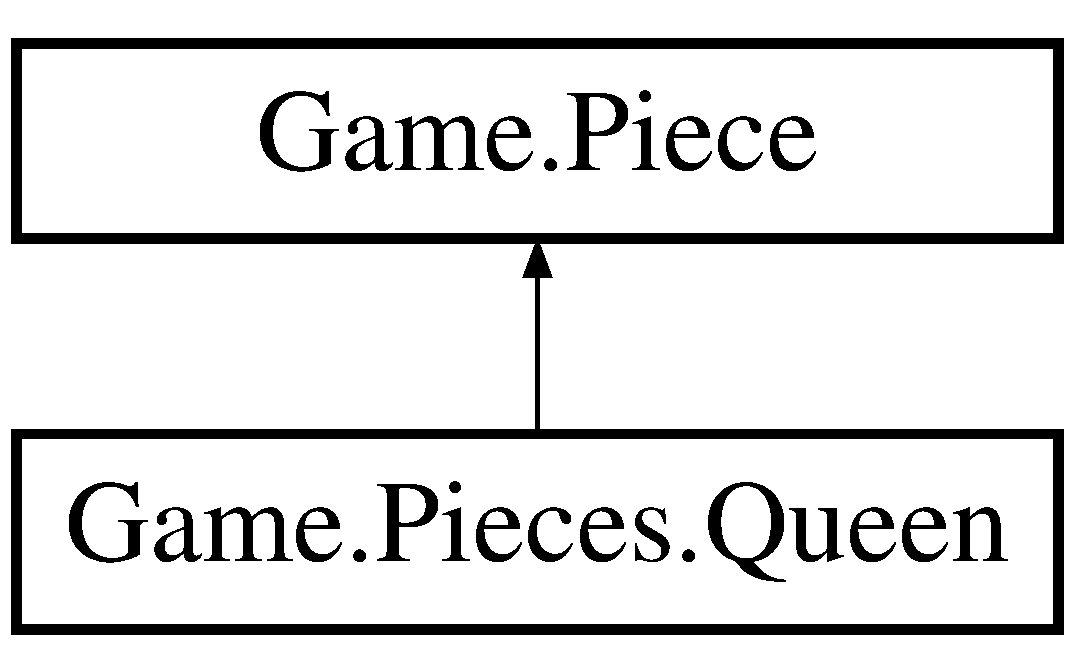
\includegraphics[height=2.000000cm]{class_game_1_1_pieces_1_1_queen}
\end{center}
\end{figure}
\subsection*{Public Member Functions}
\begin{DoxyCompactItemize}
\item 
\hyperlink{class_game_1_1_pieces_1_1_queen_af381f57ec9bc379e0da9d3caec0d5100}{Queen} (int X, int Y, int c, \hyperlink{class_game_1_1_player}{Player} owner)
\item 
Array\+List$<$ \hyperlink{class_game_1_1_location}{Location} $>$ \hyperlink{class_game_1_1_pieces_1_1_queen_a316c438998d9f78f313ebc4d02f5166f}{explore\+\_\+possible\+\_\+positions} (\hyperlink{class_game_1_1_location}{Location} location, \hyperlink{class_game_1_1_chess_board}{Chess\+Board} chess\+Board)
\end{DoxyCompactItemize}
\subsection*{Additional Inherited Members}


\subsection{Constructor \& Destructor Documentation}
\mbox{\Hypertarget{class_game_1_1_pieces_1_1_queen_af381f57ec9bc379e0da9d3caec0d5100}\label{class_game_1_1_pieces_1_1_queen_af381f57ec9bc379e0da9d3caec0d5100}} 
\index{Game\+::\+Pieces\+::\+Queen@{Game\+::\+Pieces\+::\+Queen}!Queen@{Queen}}
\index{Queen@{Queen}!Game\+::\+Pieces\+::\+Queen@{Game\+::\+Pieces\+::\+Queen}}
\subsubsection{\texorpdfstring{Queen()}{Queen()}}
{\footnotesize\ttfamily Game.\+Pieces.\+Queen.\+Queen (\begin{DoxyParamCaption}\item[{int}]{X,  }\item[{int}]{Y,  }\item[{int}]{c,  }\item[{\hyperlink{class_game_1_1_player}{Player}}]{owner }\end{DoxyParamCaption})\hspace{0.3cm}{\ttfamily [inline]}}

Constructor. 
\begin{DoxyParams}{Parameters}
{\em c} & color of piece. \\
\hline
{\em X} & X coordinate. \\
\hline
{\em Y} & y coordinate. \\
\hline
{\em owner} & is the owner of the piece. \\
\hline
\end{DoxyParams}


\subsection{Member Function Documentation}
\mbox{\Hypertarget{class_game_1_1_pieces_1_1_queen_a316c438998d9f78f313ebc4d02f5166f}\label{class_game_1_1_pieces_1_1_queen_a316c438998d9f78f313ebc4d02f5166f}} 
\index{Game\+::\+Pieces\+::\+Queen@{Game\+::\+Pieces\+::\+Queen}!explore\+\_\+possible\+\_\+positions@{explore\+\_\+possible\+\_\+positions}}
\index{explore\+\_\+possible\+\_\+positions@{explore\+\_\+possible\+\_\+positions}!Game\+::\+Pieces\+::\+Queen@{Game\+::\+Pieces\+::\+Queen}}
\subsubsection{\texorpdfstring{explore\+\_\+possible\+\_\+positions()}{explore\_possible\_positions()}}
{\footnotesize\ttfamily Array\+List$<$\hyperlink{class_game_1_1_location}{Location}$>$ Game.\+Pieces.\+Queen.\+explore\+\_\+possible\+\_\+positions (\begin{DoxyParamCaption}\item[{\hyperlink{class_game_1_1_location}{Location}}]{location,  }\item[{\hyperlink{class_game_1_1_chess_board}{Chess\+Board}}]{chess\+Board }\end{DoxyParamCaption})\hspace{0.3cm}{\ttfamily [inline]}}

Explores all options for movement from location. 
\begin{DoxyParams}{Parameters}
{\em location} & location from where we want to explore. \\
\hline
{\em chess\+Board} & is the chess board we are working on. \\
\hline
\end{DoxyParams}


The documentation for this class was generated from the following file\+:\begin{DoxyCompactItemize}
\item 
src/\+Game/\+Pieces/Queen.\+java\end{DoxyCompactItemize}

\hypertarget{class_tests_1_1_queen_test}{}\section{Tests.\+Queen\+Test Class Reference}
\label{class_tests_1_1_queen_test}\index{Tests.\+Queen\+Test@{Tests.\+Queen\+Test}}
\subsection*{Public Member Functions}
\begin{DoxyCompactItemize}
\item 
void \hyperlink{class_tests_1_1_queen_test_a23ace3b7817d95fa5e64b4a9899a5364}{can\+Move\+To\+Cell\+Incorrect\+Test} ()  throws Exception 
\item 
void \hyperlink{class_tests_1_1_queen_test_a0b52ed7e9f5c35e03c62da59a21748b1}{can\+Move\+To\+Cell\+Correct\+Test} ()  throws Exception 
\item 
void \hyperlink{class_tests_1_1_queen_test_ade9b04c6ac46fcab572c5305f71b0044}{explore\+\_\+possible\+\_\+positions\+All\+Test} ()  throws Exception 
\item 
void \hyperlink{class_tests_1_1_queen_test_afd193877a3973ecee5bedb4df0b9a8ef}{explore\+\_\+possible\+\_\+positions\+Block\+Capture\+Test} ()  throws Exception 
\end{DoxyCompactItemize}


\subsection{Member Function Documentation}
\mbox{\Hypertarget{class_tests_1_1_queen_test_a0b52ed7e9f5c35e03c62da59a21748b1}\label{class_tests_1_1_queen_test_a0b52ed7e9f5c35e03c62da59a21748b1}} 
\index{Tests\+::\+Queen\+Test@{Tests\+::\+Queen\+Test}!can\+Move\+To\+Cell\+Correct\+Test@{can\+Move\+To\+Cell\+Correct\+Test}}
\index{can\+Move\+To\+Cell\+Correct\+Test@{can\+Move\+To\+Cell\+Correct\+Test}!Tests\+::\+Queen\+Test@{Tests\+::\+Queen\+Test}}
\subsubsection{\texorpdfstring{can\+Move\+To\+Cell\+Correct\+Test()}{canMoveToCellCorrectTest()}}
{\footnotesize\ttfamily void Tests.\+Queen\+Test.\+can\+Move\+To\+Cell\+Correct\+Test (\begin{DoxyParamCaption}{ }\end{DoxyParamCaption}) throws Exception\hspace{0.3cm}{\ttfamily [inline]}}

Check if King can move to correct piece. Should return true. \mbox{\Hypertarget{class_tests_1_1_queen_test_a23ace3b7817d95fa5e64b4a9899a5364}\label{class_tests_1_1_queen_test_a23ace3b7817d95fa5e64b4a9899a5364}} 
\index{Tests\+::\+Queen\+Test@{Tests\+::\+Queen\+Test}!can\+Move\+To\+Cell\+Incorrect\+Test@{can\+Move\+To\+Cell\+Incorrect\+Test}}
\index{can\+Move\+To\+Cell\+Incorrect\+Test@{can\+Move\+To\+Cell\+Incorrect\+Test}!Tests\+::\+Queen\+Test@{Tests\+::\+Queen\+Test}}
\subsubsection{\texorpdfstring{can\+Move\+To\+Cell\+Incorrect\+Test()}{canMoveToCellIncorrectTest()}}
{\footnotesize\ttfamily void Tests.\+Queen\+Test.\+can\+Move\+To\+Cell\+Incorrect\+Test (\begin{DoxyParamCaption}{ }\end{DoxyParamCaption}) throws Exception\hspace{0.3cm}{\ttfamily [inline]}}

Check if King can move to incorrect piece. Should return false. \mbox{\Hypertarget{class_tests_1_1_queen_test_ade9b04c6ac46fcab572c5305f71b0044}\label{class_tests_1_1_queen_test_ade9b04c6ac46fcab572c5305f71b0044}} 
\index{Tests\+::\+Queen\+Test@{Tests\+::\+Queen\+Test}!explore\+\_\+possible\+\_\+positions\+All\+Test@{explore\+\_\+possible\+\_\+positions\+All\+Test}}
\index{explore\+\_\+possible\+\_\+positions\+All\+Test@{explore\+\_\+possible\+\_\+positions\+All\+Test}!Tests\+::\+Queen\+Test@{Tests\+::\+Queen\+Test}}
\subsubsection{\texorpdfstring{explore\+\_\+possible\+\_\+positions\+All\+Test()}{explore\_possible\_positionsAllTest()}}
{\footnotesize\ttfamily void Tests.\+Queen\+Test.\+explore\+\_\+possible\+\_\+positions\+All\+Test (\begin{DoxyParamCaption}{ }\end{DoxyParamCaption}) throws Exception\hspace{0.3cm}{\ttfamily [inline]}}

Return all the places that a Queen can go from a position with no other pieces on board. \mbox{\Hypertarget{class_tests_1_1_queen_test_afd193877a3973ecee5bedb4df0b9a8ef}\label{class_tests_1_1_queen_test_afd193877a3973ecee5bedb4df0b9a8ef}} 
\index{Tests\+::\+Queen\+Test@{Tests\+::\+Queen\+Test}!explore\+\_\+possible\+\_\+positions\+Block\+Capture\+Test@{explore\+\_\+possible\+\_\+positions\+Block\+Capture\+Test}}
\index{explore\+\_\+possible\+\_\+positions\+Block\+Capture\+Test@{explore\+\_\+possible\+\_\+positions\+Block\+Capture\+Test}!Tests\+::\+Queen\+Test@{Tests\+::\+Queen\+Test}}
\subsubsection{\texorpdfstring{explore\+\_\+possible\+\_\+positions\+Block\+Capture\+Test()}{explore\_possible\_positionsBlockCaptureTest()}}
{\footnotesize\ttfamily void Tests.\+Queen\+Test.\+explore\+\_\+possible\+\_\+positions\+Block\+Capture\+Test (\begin{DoxyParamCaption}{ }\end{DoxyParamCaption}) throws Exception\hspace{0.3cm}{\ttfamily [inline]}}

Return all the places that a Queen can go from a position with some other pieces on board. 

The documentation for this class was generated from the following file\+:\begin{DoxyCompactItemize}
\item 
src/\+Tests/Queen\+Test.\+java\end{DoxyCompactItemize}

\hypertarget{class_game_1_1_pieces_1_1_rook}{}\section{Game.\+Pieces.\+Rook Class Reference}
\label{class_game_1_1_pieces_1_1_rook}\index{Game.\+Pieces.\+Rook@{Game.\+Pieces.\+Rook}}
Inheritance diagram for Game.\+Pieces.\+Rook\+:\begin{figure}[H]
\begin{center}
\leavevmode
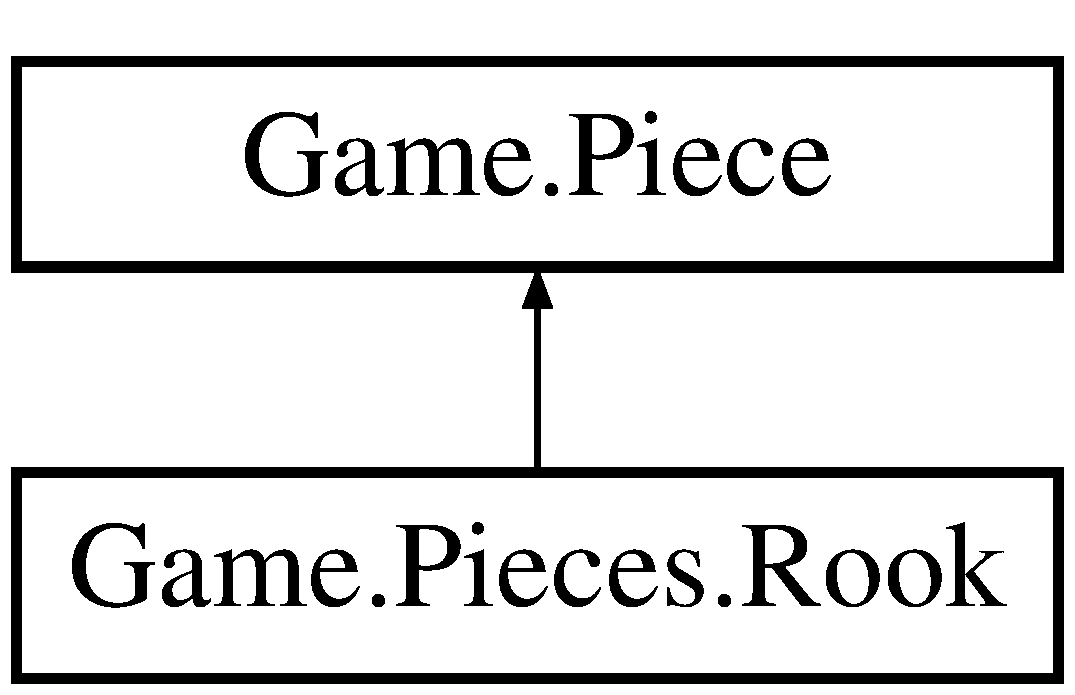
\includegraphics[height=2.000000cm]{class_game_1_1_pieces_1_1_rook}
\end{center}
\end{figure}
\subsection*{Public Member Functions}
\begin{DoxyCompactItemize}
\item 
\hyperlink{class_game_1_1_pieces_1_1_rook_a30976d18bff9d0dae46e7b5edd89eaaf}{Rook} (int X, int Y, int c, \hyperlink{class_game_1_1_player}{Player} owner)
\item 
Array\+List$<$ \hyperlink{class_game_1_1_location}{Location} $>$ \hyperlink{class_game_1_1_pieces_1_1_rook_a624cb321b47a960b392211b3da8d0b7c}{explore\+\_\+possible\+\_\+positions} (\hyperlink{class_game_1_1_location}{Location} location, \hyperlink{class_game_1_1_chess_board}{Chess\+Board} chess\+Board)
\end{DoxyCompactItemize}
\subsection*{Additional Inherited Members}


\subsection{Constructor \& Destructor Documentation}
\mbox{\Hypertarget{class_game_1_1_pieces_1_1_rook_a30976d18bff9d0dae46e7b5edd89eaaf}\label{class_game_1_1_pieces_1_1_rook_a30976d18bff9d0dae46e7b5edd89eaaf}} 
\index{Game\+::\+Pieces\+::\+Rook@{Game\+::\+Pieces\+::\+Rook}!Rook@{Rook}}
\index{Rook@{Rook}!Game\+::\+Pieces\+::\+Rook@{Game\+::\+Pieces\+::\+Rook}}
\subsubsection{\texorpdfstring{Rook()}{Rook()}}
{\footnotesize\ttfamily Game.\+Pieces.\+Rook.\+Rook (\begin{DoxyParamCaption}\item[{int}]{X,  }\item[{int}]{Y,  }\item[{int}]{c,  }\item[{\hyperlink{class_game_1_1_player}{Player}}]{owner }\end{DoxyParamCaption})\hspace{0.3cm}{\ttfamily [inline]}}

Adds all valid moves in a straight line to the list. Valid here means, on board and capturable or unoccupied. 
\begin{DoxyParams}{Parameters}
{\em c} & color of piece. \\
\hline
{\em X} & X coordinate. \\
\hline
{\em Y} & y coordinate. \\
\hline
{\em owner} & is the owner of the piece. \\
\hline
\end{DoxyParams}


\subsection{Member Function Documentation}
\mbox{\Hypertarget{class_game_1_1_pieces_1_1_rook_a624cb321b47a960b392211b3da8d0b7c}\label{class_game_1_1_pieces_1_1_rook_a624cb321b47a960b392211b3da8d0b7c}} 
\index{Game\+::\+Pieces\+::\+Rook@{Game\+::\+Pieces\+::\+Rook}!explore\+\_\+possible\+\_\+positions@{explore\+\_\+possible\+\_\+positions}}
\index{explore\+\_\+possible\+\_\+positions@{explore\+\_\+possible\+\_\+positions}!Game\+::\+Pieces\+::\+Rook@{Game\+::\+Pieces\+::\+Rook}}
\subsubsection{\texorpdfstring{explore\+\_\+possible\+\_\+positions()}{explore\_possible\_positions()}}
{\footnotesize\ttfamily Array\+List$<$\hyperlink{class_game_1_1_location}{Location}$>$ Game.\+Pieces.\+Rook.\+explore\+\_\+possible\+\_\+positions (\begin{DoxyParamCaption}\item[{\hyperlink{class_game_1_1_location}{Location}}]{location,  }\item[{\hyperlink{class_game_1_1_chess_board}{Chess\+Board}}]{chess\+Board }\end{DoxyParamCaption})\hspace{0.3cm}{\ttfamily [inline]}}

Explores all options for movement from location. 
\begin{DoxyParams}{Parameters}
{\em location} & location from where we want to explore. \\
\hline
{\em chess\+Board} & is the chess board we are working on. \\
\hline
\end{DoxyParams}


The documentation for this class was generated from the following file\+:\begin{DoxyCompactItemize}
\item 
src/\+Game/\+Pieces/Rook.\+java\end{DoxyCompactItemize}

\hypertarget{class_tests_1_1_rook_test}{}\section{Tests.\+Rook\+Test Class Reference}
\label{class_tests_1_1_rook_test}\index{Tests.\+Rook\+Test@{Tests.\+Rook\+Test}}
\subsection*{Public Member Functions}
\begin{DoxyCompactItemize}
\item 
void \hyperlink{class_tests_1_1_rook_test_af0973359c90be81d5789430155def5d5}{can\+Move\+To\+Cell\+Incorrect\+Test} ()  throws Exception 
\item 
void \hyperlink{class_tests_1_1_rook_test_a02bb2ab60818cd4d1746f37c31e70ecc}{can\+Move\+To\+Cell\+Correct\+Test} ()  throws Exception 
\item 
void \hyperlink{class_tests_1_1_rook_test_a53cd669ac179cb3c550cb862b09374c0}{explore\+\_\+possible\+\_\+positions\+All\+Test} ()  throws Exception 
\item 
void \hyperlink{class_tests_1_1_rook_test_ac9c944f9e194ae63eebfff8ff99a0284}{explore\+\_\+possible\+\_\+positions\+Block\+Capture\+Test} ()  throws Exception 
\end{DoxyCompactItemize}


\subsection{Member Function Documentation}
\mbox{\Hypertarget{class_tests_1_1_rook_test_a02bb2ab60818cd4d1746f37c31e70ecc}\label{class_tests_1_1_rook_test_a02bb2ab60818cd4d1746f37c31e70ecc}} 
\index{Tests\+::\+Rook\+Test@{Tests\+::\+Rook\+Test}!can\+Move\+To\+Cell\+Correct\+Test@{can\+Move\+To\+Cell\+Correct\+Test}}
\index{can\+Move\+To\+Cell\+Correct\+Test@{can\+Move\+To\+Cell\+Correct\+Test}!Tests\+::\+Rook\+Test@{Tests\+::\+Rook\+Test}}
\subsubsection{\texorpdfstring{can\+Move\+To\+Cell\+Correct\+Test()}{canMoveToCellCorrectTest()}}
{\footnotesize\ttfamily void Tests.\+Rook\+Test.\+can\+Move\+To\+Cell\+Correct\+Test (\begin{DoxyParamCaption}{ }\end{DoxyParamCaption}) throws Exception\hspace{0.3cm}{\ttfamily [inline]}}

Check if King can move to correct piece. Should return true. \mbox{\Hypertarget{class_tests_1_1_rook_test_af0973359c90be81d5789430155def5d5}\label{class_tests_1_1_rook_test_af0973359c90be81d5789430155def5d5}} 
\index{Tests\+::\+Rook\+Test@{Tests\+::\+Rook\+Test}!can\+Move\+To\+Cell\+Incorrect\+Test@{can\+Move\+To\+Cell\+Incorrect\+Test}}
\index{can\+Move\+To\+Cell\+Incorrect\+Test@{can\+Move\+To\+Cell\+Incorrect\+Test}!Tests\+::\+Rook\+Test@{Tests\+::\+Rook\+Test}}
\subsubsection{\texorpdfstring{can\+Move\+To\+Cell\+Incorrect\+Test()}{canMoveToCellIncorrectTest()}}
{\footnotesize\ttfamily void Tests.\+Rook\+Test.\+can\+Move\+To\+Cell\+Incorrect\+Test (\begin{DoxyParamCaption}{ }\end{DoxyParamCaption}) throws Exception\hspace{0.3cm}{\ttfamily [inline]}}

Check if King can move to incorrect piece. Should return false. \mbox{\Hypertarget{class_tests_1_1_rook_test_a53cd669ac179cb3c550cb862b09374c0}\label{class_tests_1_1_rook_test_a53cd669ac179cb3c550cb862b09374c0}} 
\index{Tests\+::\+Rook\+Test@{Tests\+::\+Rook\+Test}!explore\+\_\+possible\+\_\+positions\+All\+Test@{explore\+\_\+possible\+\_\+positions\+All\+Test}}
\index{explore\+\_\+possible\+\_\+positions\+All\+Test@{explore\+\_\+possible\+\_\+positions\+All\+Test}!Tests\+::\+Rook\+Test@{Tests\+::\+Rook\+Test}}
\subsubsection{\texorpdfstring{explore\+\_\+possible\+\_\+positions\+All\+Test()}{explore\_possible\_positionsAllTest()}}
{\footnotesize\ttfamily void Tests.\+Rook\+Test.\+explore\+\_\+possible\+\_\+positions\+All\+Test (\begin{DoxyParamCaption}{ }\end{DoxyParamCaption}) throws Exception\hspace{0.3cm}{\ttfamily [inline]}}

Return all the places that a Rook can go from a position with no other pieces on board. \mbox{\Hypertarget{class_tests_1_1_rook_test_ac9c944f9e194ae63eebfff8ff99a0284}\label{class_tests_1_1_rook_test_ac9c944f9e194ae63eebfff8ff99a0284}} 
\index{Tests\+::\+Rook\+Test@{Tests\+::\+Rook\+Test}!explore\+\_\+possible\+\_\+positions\+Block\+Capture\+Test@{explore\+\_\+possible\+\_\+positions\+Block\+Capture\+Test}}
\index{explore\+\_\+possible\+\_\+positions\+Block\+Capture\+Test@{explore\+\_\+possible\+\_\+positions\+Block\+Capture\+Test}!Tests\+::\+Rook\+Test@{Tests\+::\+Rook\+Test}}
\subsubsection{\texorpdfstring{explore\+\_\+possible\+\_\+positions\+Block\+Capture\+Test()}{explore\_possible\_positionsBlockCaptureTest()}}
{\footnotesize\ttfamily void Tests.\+Rook\+Test.\+explore\+\_\+possible\+\_\+positions\+Block\+Capture\+Test (\begin{DoxyParamCaption}{ }\end{DoxyParamCaption}) throws Exception\hspace{0.3cm}{\ttfamily [inline]}}

Return all the places that a Rook can go from a position with some other pieces on board. 

The documentation for this class was generated from the following file\+:\begin{DoxyCompactItemize}
\item 
src/\+Tests/Rook\+Test.\+java\end{DoxyCompactItemize}

%--- End generated contents ---

% Index
\backmatter
\newpage
\phantomsection
\clearemptydoublepage
\addcontentsline{toc}{chapter}{Index}
\printindex

\end{document}
